\chapter{Quasar Emission Lines as Probes of Orientation and Unification}



{\em This chapter is based on a paper in prepation:

Matthews J. H., Knigge C., 
`Quasar Emission Lines as Probes of Orientation and Unification',
to be submitted to MNRAS.}


%%%%%%%%%%%%%%%%%%%%%%%%%%%%%%%%%%%%%%
%
%          ABSTRACT
%
%%%%%%%%%%%%%%%%%%%%%%%%%%%%%%%%%%%%%%%
\maketitle

\section{Introduction}

In the previous chapter, I presented tests of geometric unification
models using MCRT and photoionization simulations. 
One of the key results from that analysis is that trends with
inclination prohibit models with equatorial outflows matching
observations, as the EW of the emission lines tend
to increase with inclination. This trend has clear implications for
the geometries of BAL outflows; the viewing angle may determine many
of the selection effects at work and must therefore be understood
before the true covering factor of BAL outflows can be accurately 
determined. The covering factor and opening angle of the outflow
are important quantities to measure in order to calculate the
feedback efficiency \citep[e.g.][]{borguet2012}, 
and understand the outflow physics \citep[e.g.][]{proga2005}. 

Unlike in galactic accretion disc systems, measuring inclinations
for quasars and AGN is notoriously difficult, and obtaining 
reliable orientation indicators is thus an important observational
goal for the community. Perhaps as a result of this problem, 
directly opposing geometries have been proposed for 
BAL outflows (see section~??). Here, I use observational 
data from the Sloan Digital Sky Survey to constrain the inclinations
of BAL quasars. Similar attempts have been made previously with
different diagnostics; for example, by considering 
radio measurements \citep{zhou2006,dipompeo2012a}, 
polarisation \citep{brotherton2006}
and emission line properties \citep{dipompeo2012b}.  

This chapter is structured as follows. First, I describe
the data sample and selection criteria being used. I begin by
simply examining the distributions of the EW of the \oiiifull\ emission line,
\ewo, and comparing the BAL and non-BAL quasar distributions. 
In section~\ref{sec:disc_agn} I review the angular distribution of 
continuum emission one would expect from simple $\alpha$-disc models, 
as well as exploring more advanced disc models computed
with \agn. I then use these theoretical 
angular distributions applied to a simple toy model in 
section~\ref{sec:mc_angular},
and conduct MC simulations in an attempt to fit the observed LoBAL and non-BAL
quasar distributions of \ewo, using a similar approach to 
\cite{risaliti2011}. I also discuss the broad emission
line distribution in HiBAL quasars more detail in this section. 
In section~\ref{sec:discuss_ew} I discuss the results
in the context of radio and polarisation measurements of AGN, as well
as exploring the location of BAL quasars in `Eigenvector 1' parameter space.
Finally, in section~\ref{sec:ew_conclusions}, I summarise the results.

% {\bf{\sl{\huge Abstract}}}

% The incidence of broad absorption lines (BALs) in quasar samples is 
% often explained by a geometric unification model consisting
% of an accretion disc and an associated outflow.
% This outflows is assumed to have a covering factor roughly equivalent to
% the BAL fraction, $f_{BAL}$. We test this model
% by examining ultraviolet (UV) emission line equivalent-widths. 
% We find that a model in which the 
% continuum emission arises from a geometrically thin, 
% optically thick accretion disc is inconsistent with this property
% unless (i) the line emission has the same angular distribution of 
% emission as the continuum or (ii) BAL quasars are viewed from a low or intermediate inclination. 
% We examine whether an accretion disc can emit isotropically, and
% demonstrate that general relativistic effects cannot sufficiently isotropise the 
% radiation field in the UV. 
% We suggest that reprocessing by outflows, or limb brightening due to X-ray irradiation, may play a role.
% We then explore in what limits line emission can emit with the same angular
% distribution as a foreshortened, limb-darkened disc, and discuss our results
% in the context of other observational studies of broad emission line 
% equivalent-widths in quasars.
% Finally we explore geometries in which BAL quasars are viewed
% from a low or intermediate inclination with reference to polarisation
% and modelling results. We also discuss the effect of the outflow 
% geometry on the inferred BAL fraction. We favour a scenario in which the 
% BAL outflow is {\em not} equatorial, and BAL quasars
% are instead viewed from $\sim45^\circ$ as suggested from radio measurements,
% but a number of open questions remain.

% \clearpage

%%%%%%%%%%%%%%%%%%%%%%%%%%%%%%%%%%%%%%
%
%          INTRODUCTION
%
%%%%%%%%%%%%%%%%%%%%%%%%%%%%%%%%%%%%%%%

%{\em This chapter is based on a paper in preparation of the same title, 
%due to be submitted to MNRAS.}

%\section{Introduction}
% {\color{blue}
% Introduction to the topic, particular relating to unification
% and BAL geometries. At the moment this is a placeholder.
% }
% \bigskip

%\noindent
% A number of quasar unification schemes have attempted to explain 
% the incidence of BAL quasars in terms of an outflow which rises 
% from an accretion disc \citep[e.g.][]{MCGV95, elvis2000}. 
% The covering factor of this outflow is then
% expected to determine the BAL fraction, $f_{BAL}$, thought to be
% between $20\%$ and $40\%$ 
% \citep{weymann1991, reichard2003, knigge2008, allen2011}.
% These outflows are of wide-reaching astrophysical significance as 
% they may be an efficient way for the central accretion engine to interact
% with its galactic environment (REFs), potentially explaining 
% for the $M-\sigma$ relation (REFs).

% Unlike in galactic accretion disc systems, measuring inclinations
% for quasars and AGN is notoriously difficult, and obtaining 
% reliable orientation indicators is thus an important observational
% goal for the community. Directly opposing 
% geometries have been proposed for BAL outflows, mostly from observations
% of radio-loud sources. A number of polarisation
% studies of BALQSOs have measured large angle differences 
% from the radio jet, implying an equatorial viewing angle 
% \citep{goodrich1995, cohen1995,brotherton2006}.
% Conversely, Punsly (1991) suggests a polar geometry.
% This is supported by very high brightness temperatures 
% in some RL BALQSOs \citep{zhou2006} 
% and the fact that RL BALQSOs possess similar radio spectral 
% indices to normal RL quasars \citep{bruni2012}.  
% In addition, \cite{marin2013} find a bending angle of 
% $\sim45^\circ$ is required to 
% explain the polarisation dichotomy of type 1 and 2 AGN using an Elvis-type wind 
% model (Elvis 2000) --  a conclusion which is potentially extendable to BAL quasars.

% BALQSOs and quasars generally possess remarkably similar emission line properties 
% \citep[e.g.][]{weymann1991,reichard2003}. This, along with Occam's razor (see figure 1),
% is one of the reasons why they are thought to be drawn from the same population 
% as non-BAL quasars. In this paper, we start by verifying the uniformity 
% of emission line properties
% between BAL and non-BAL quasars. We then derive relationships for
% the expected angular distribution of emission for accretion discs 
% (section~\ref{disc}) and emission lines (section~\ref{lines}). Finally, we discuss
% these results in the context of unification models and offer 
% a number of possible scenarios.

% In the previous chapters we have explored quasar unification schemes
% in which the incidence of BAL quasars is explained in terms of an outflow which rises 
% from an accretion disc \citep[e.g.][]{MCGV95, elvis2000}. In chapter 5,
% we found that a biconical wind model can reproduce much of the qualitative 
% behaviour expected from a unified model, with some shortcomings. 
% In particular, we found an angular dependence of emission-line equivalent 
% width (EW), such that the EWs were much stronger at high inclination.
% Here, we attack the problem from a different angle (but informed by the 
% previous study), by examining UV and optical emission lines from the Sloan Digital Sky 
% Survey and the potential effects of orientation on their EW distributions.

% Unlike in galactic accretion disc systems, measuring inclinations
% for quasars and AGN is notoriously difficult, and obtaining 
% reliable orientation indicators is thus an important observational
% goal for the community. Directly opposing 
% geometries have been proposed for BAL outflows, mostly from observations
% of radio-loud sources. A number of polarisation
% studies of BALQSOs have measured large angle differences 
% from the radio jet, implying an equatorial viewing angle 
% \citep{goodrich1995, cohen1995,brotherton2006}.
% Conversely, Punsly (1991) suggests a polar geometry.
% This is supported by very high brightness temperatures 
% in some RL BALQSOs \citep{zhou2006} 
% and the fact that RL BALQSOs possess similar radio spectral 
% indices to normal RL quasars \citep{bruni2012}.  
% In addition, \cite{marin2013} find a bending angle of $\sim45^\circ$ is required to 
% explain the polarisation dichotomy of type 1 and 2 AGN using an \cite{elvis2000} wind 
% model --  a conclusion which is potentially extendable to BAL quasars.



\section{Data Sample}
% {\color{blue}
% First we need to show that emission line properties of 
% quasars and BAL quasars really are similar. Do that with histograms 
% of EWs. We will probably show a mixture of emission lines so we cover
% allowed dipole, forbidden and intercombination lines. 

% Questions:

% \begin{itemize}
% 	\item Do we need some kind of test statistic here? e.g. K-S
% 	\item Perhaps we should derive theoretical quasar distribution with different 
% 		  inclination cutoffs?
%     \item Do we want to repeat the analysis of Risaliti et al? 
%     \item It may make sense to start with theory, derive model distributions and 
%     	  then test them against real distributions for different physical models
%     	  and inclination cutoffs?
% \end{itemize}
% }
% \begin{figure*} %fullpage
% \centering
% 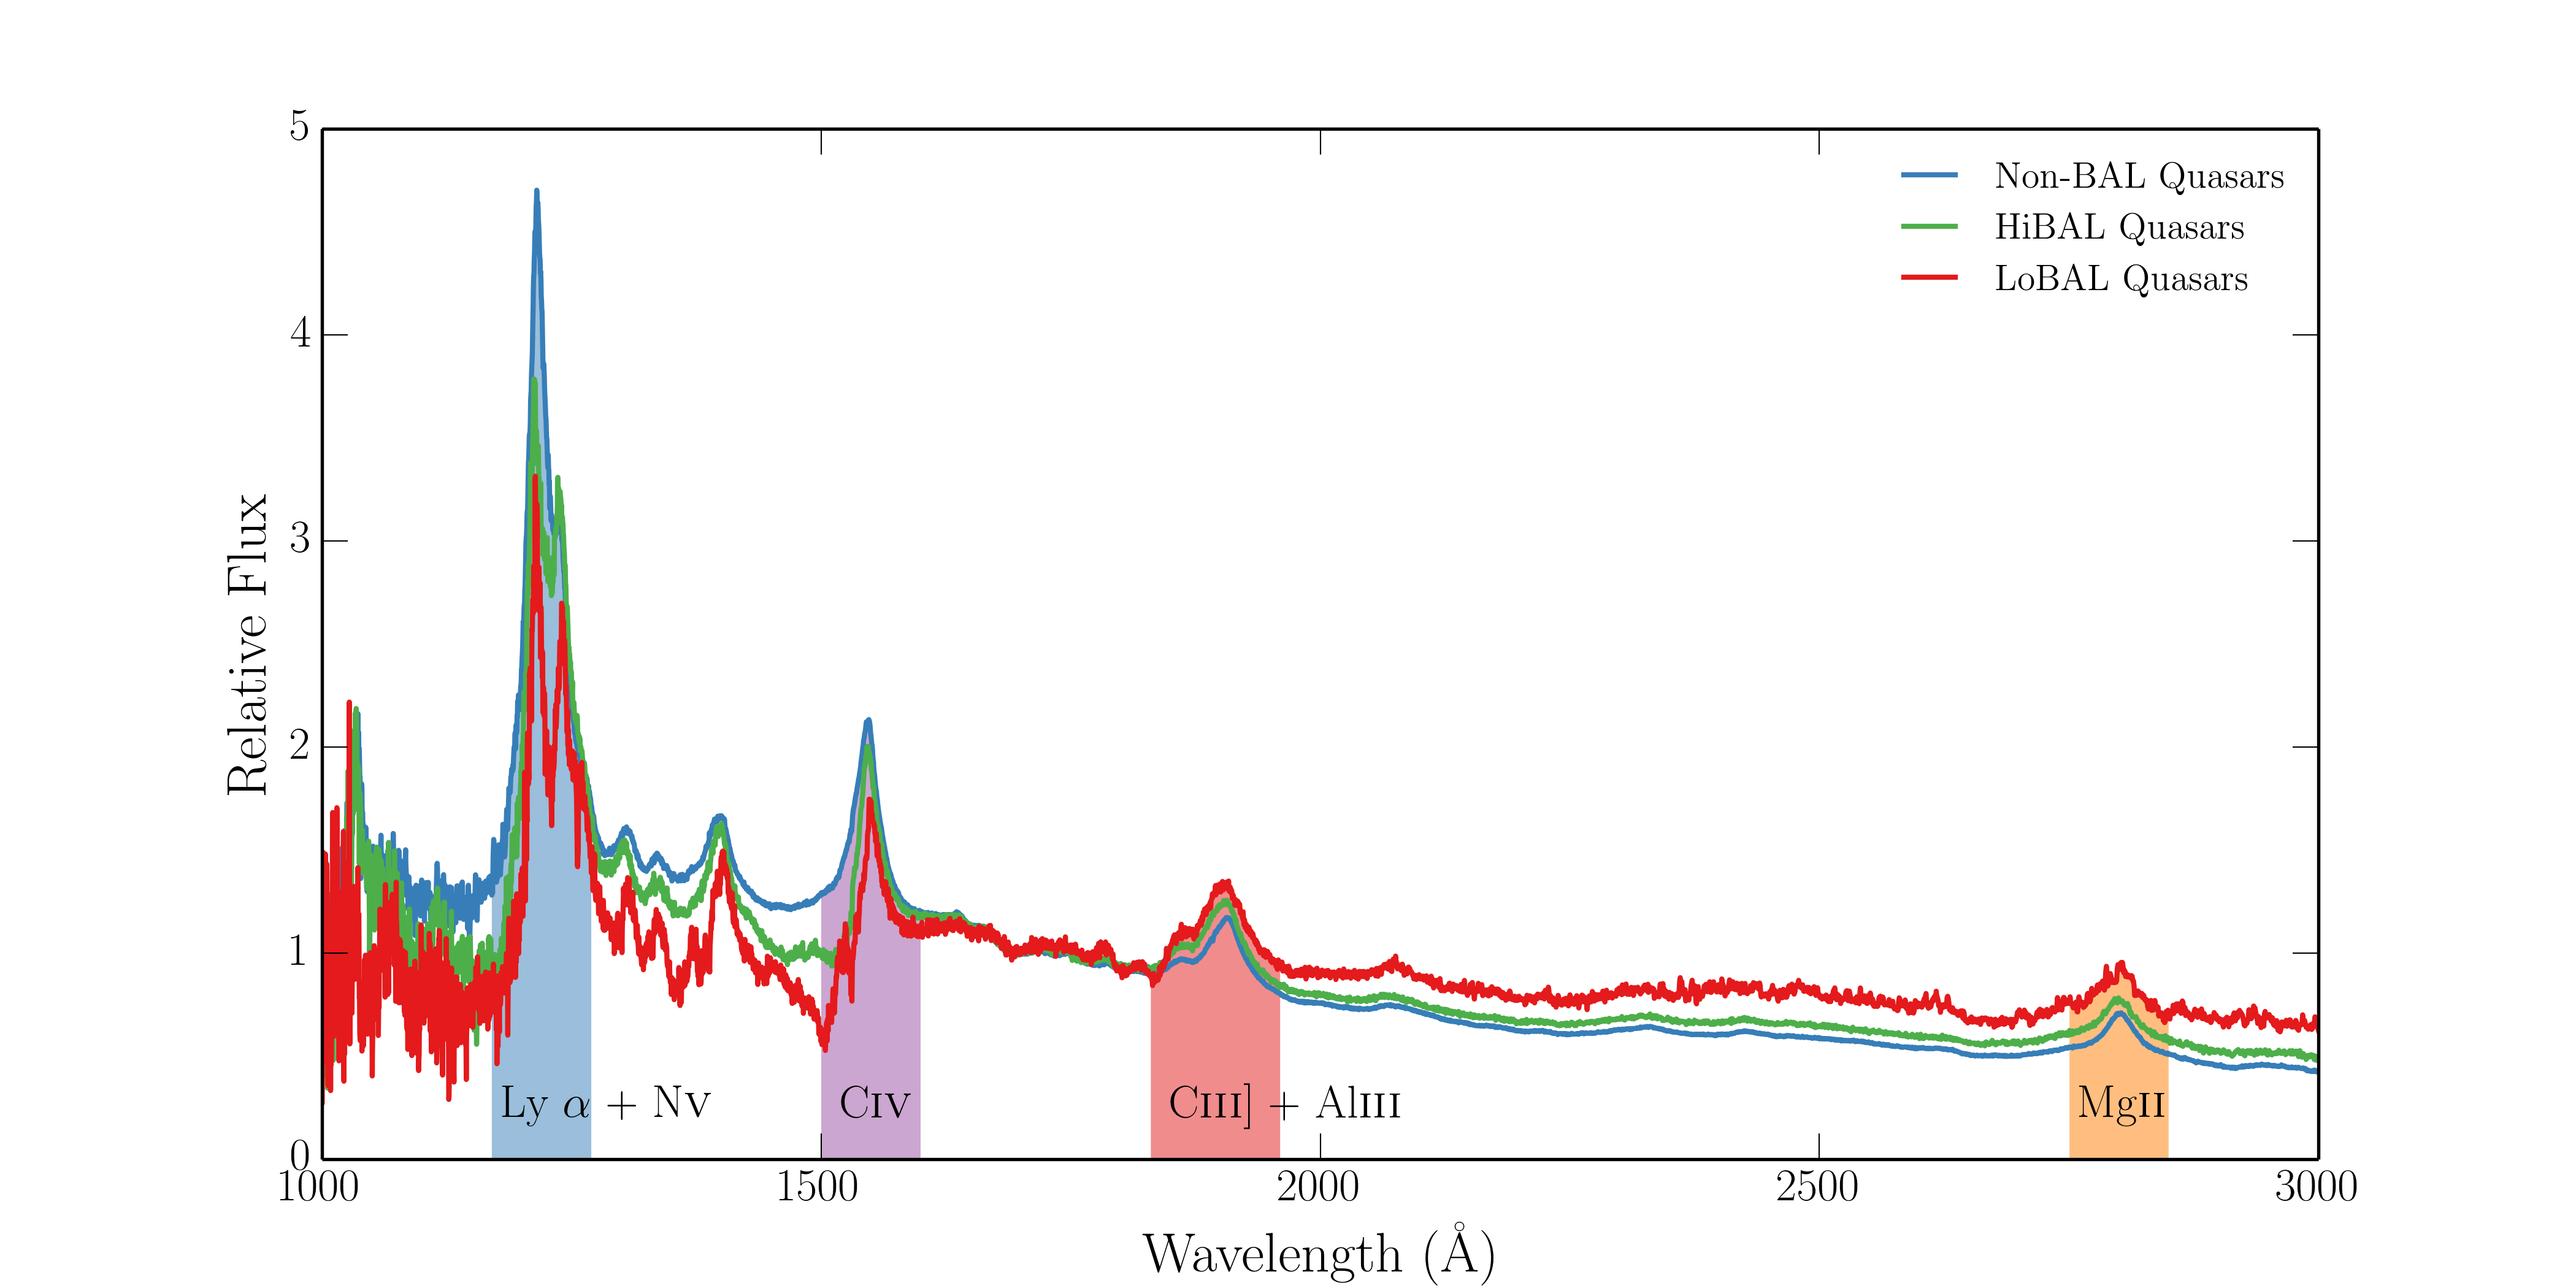
\includegraphics[width=1.0\textwidth]{figures/ewpaper/composites.png}
% \caption
% {
% SDSS Composite spectra
% }
% \label{fig:composite}
% \end{figure*} %fullpage
% The Sloan Digital Sky Survey DR7 contains ~10,000 objects in its quasar
% catalog. Many of these have been fitted with quasar templates, allowing 
% easy comparison of the equivalent width properties between the BAL and 
% non-BAL subsamples. Figure 2 shows histograms of a number of different 
% emission line properties. As found by previous authors, we find that BAL
% and non-BAL quasars really do seem to possess very similar emission line 
% properties.

% \begin{table}
% \begin{tabular}{p{2cm}p{1cm}p{1cm}p{1cm}p{1cm}}
% Sample & Redshift Range & Number of non-BAL Objects & Number of BAL objects & Number of LoBAL objects \\
% \hline \hline 
% A & $?<z<?$ & 
% \hline 
% \end{tabular}
% \caption{
% The properties of our subsamples, built from the SDSS DR7
% quasar catalog.
% }
% \label{tab:samples}
% \end{table}

\begin{figure*} %fullpage
\centering
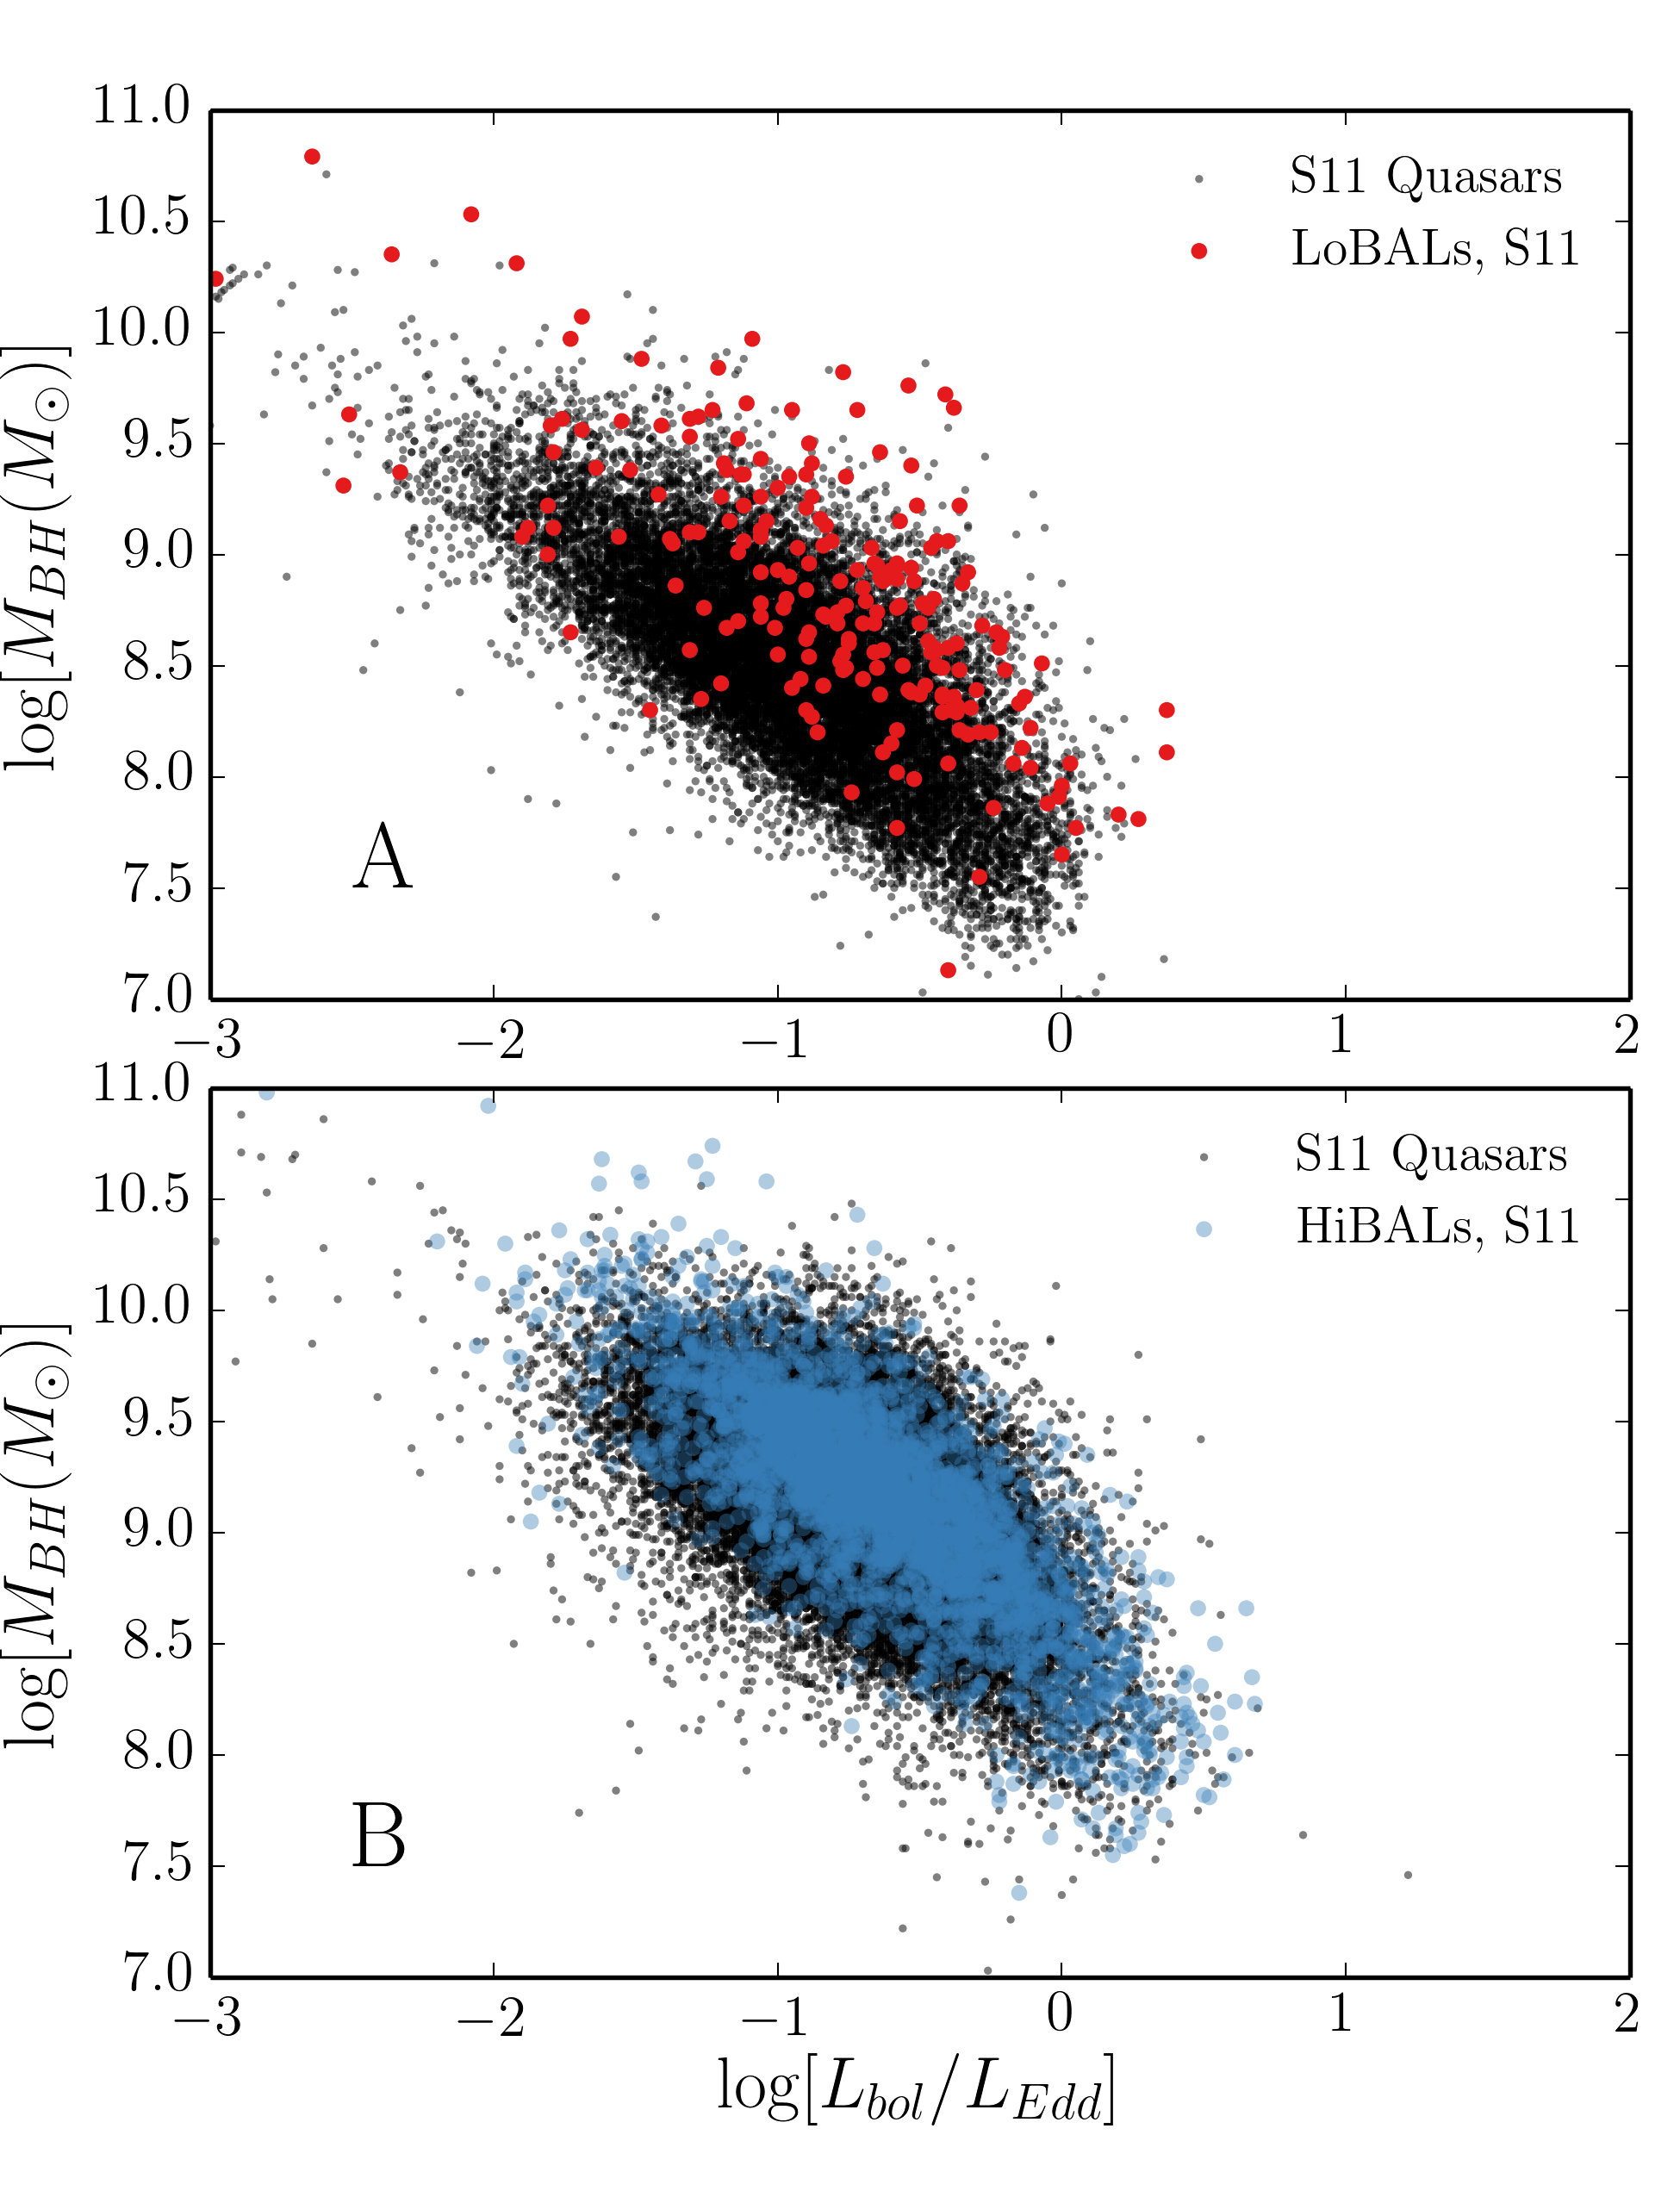
\includegraphics[width=1.0\textwidth]{figures/ewpaper/bals_2x2_scatter.png}
\caption
{
BH mass and Eddington fraction measurements from S11 for Sample A (top)
and Sample B (bottom). The LoBALs in sample A and BALs in Sample B are
also plotted in each case.
}
\label{fig:bal_scatter}
\end{figure*} %fullpage

\begin{figure*} %fullpage
\centering
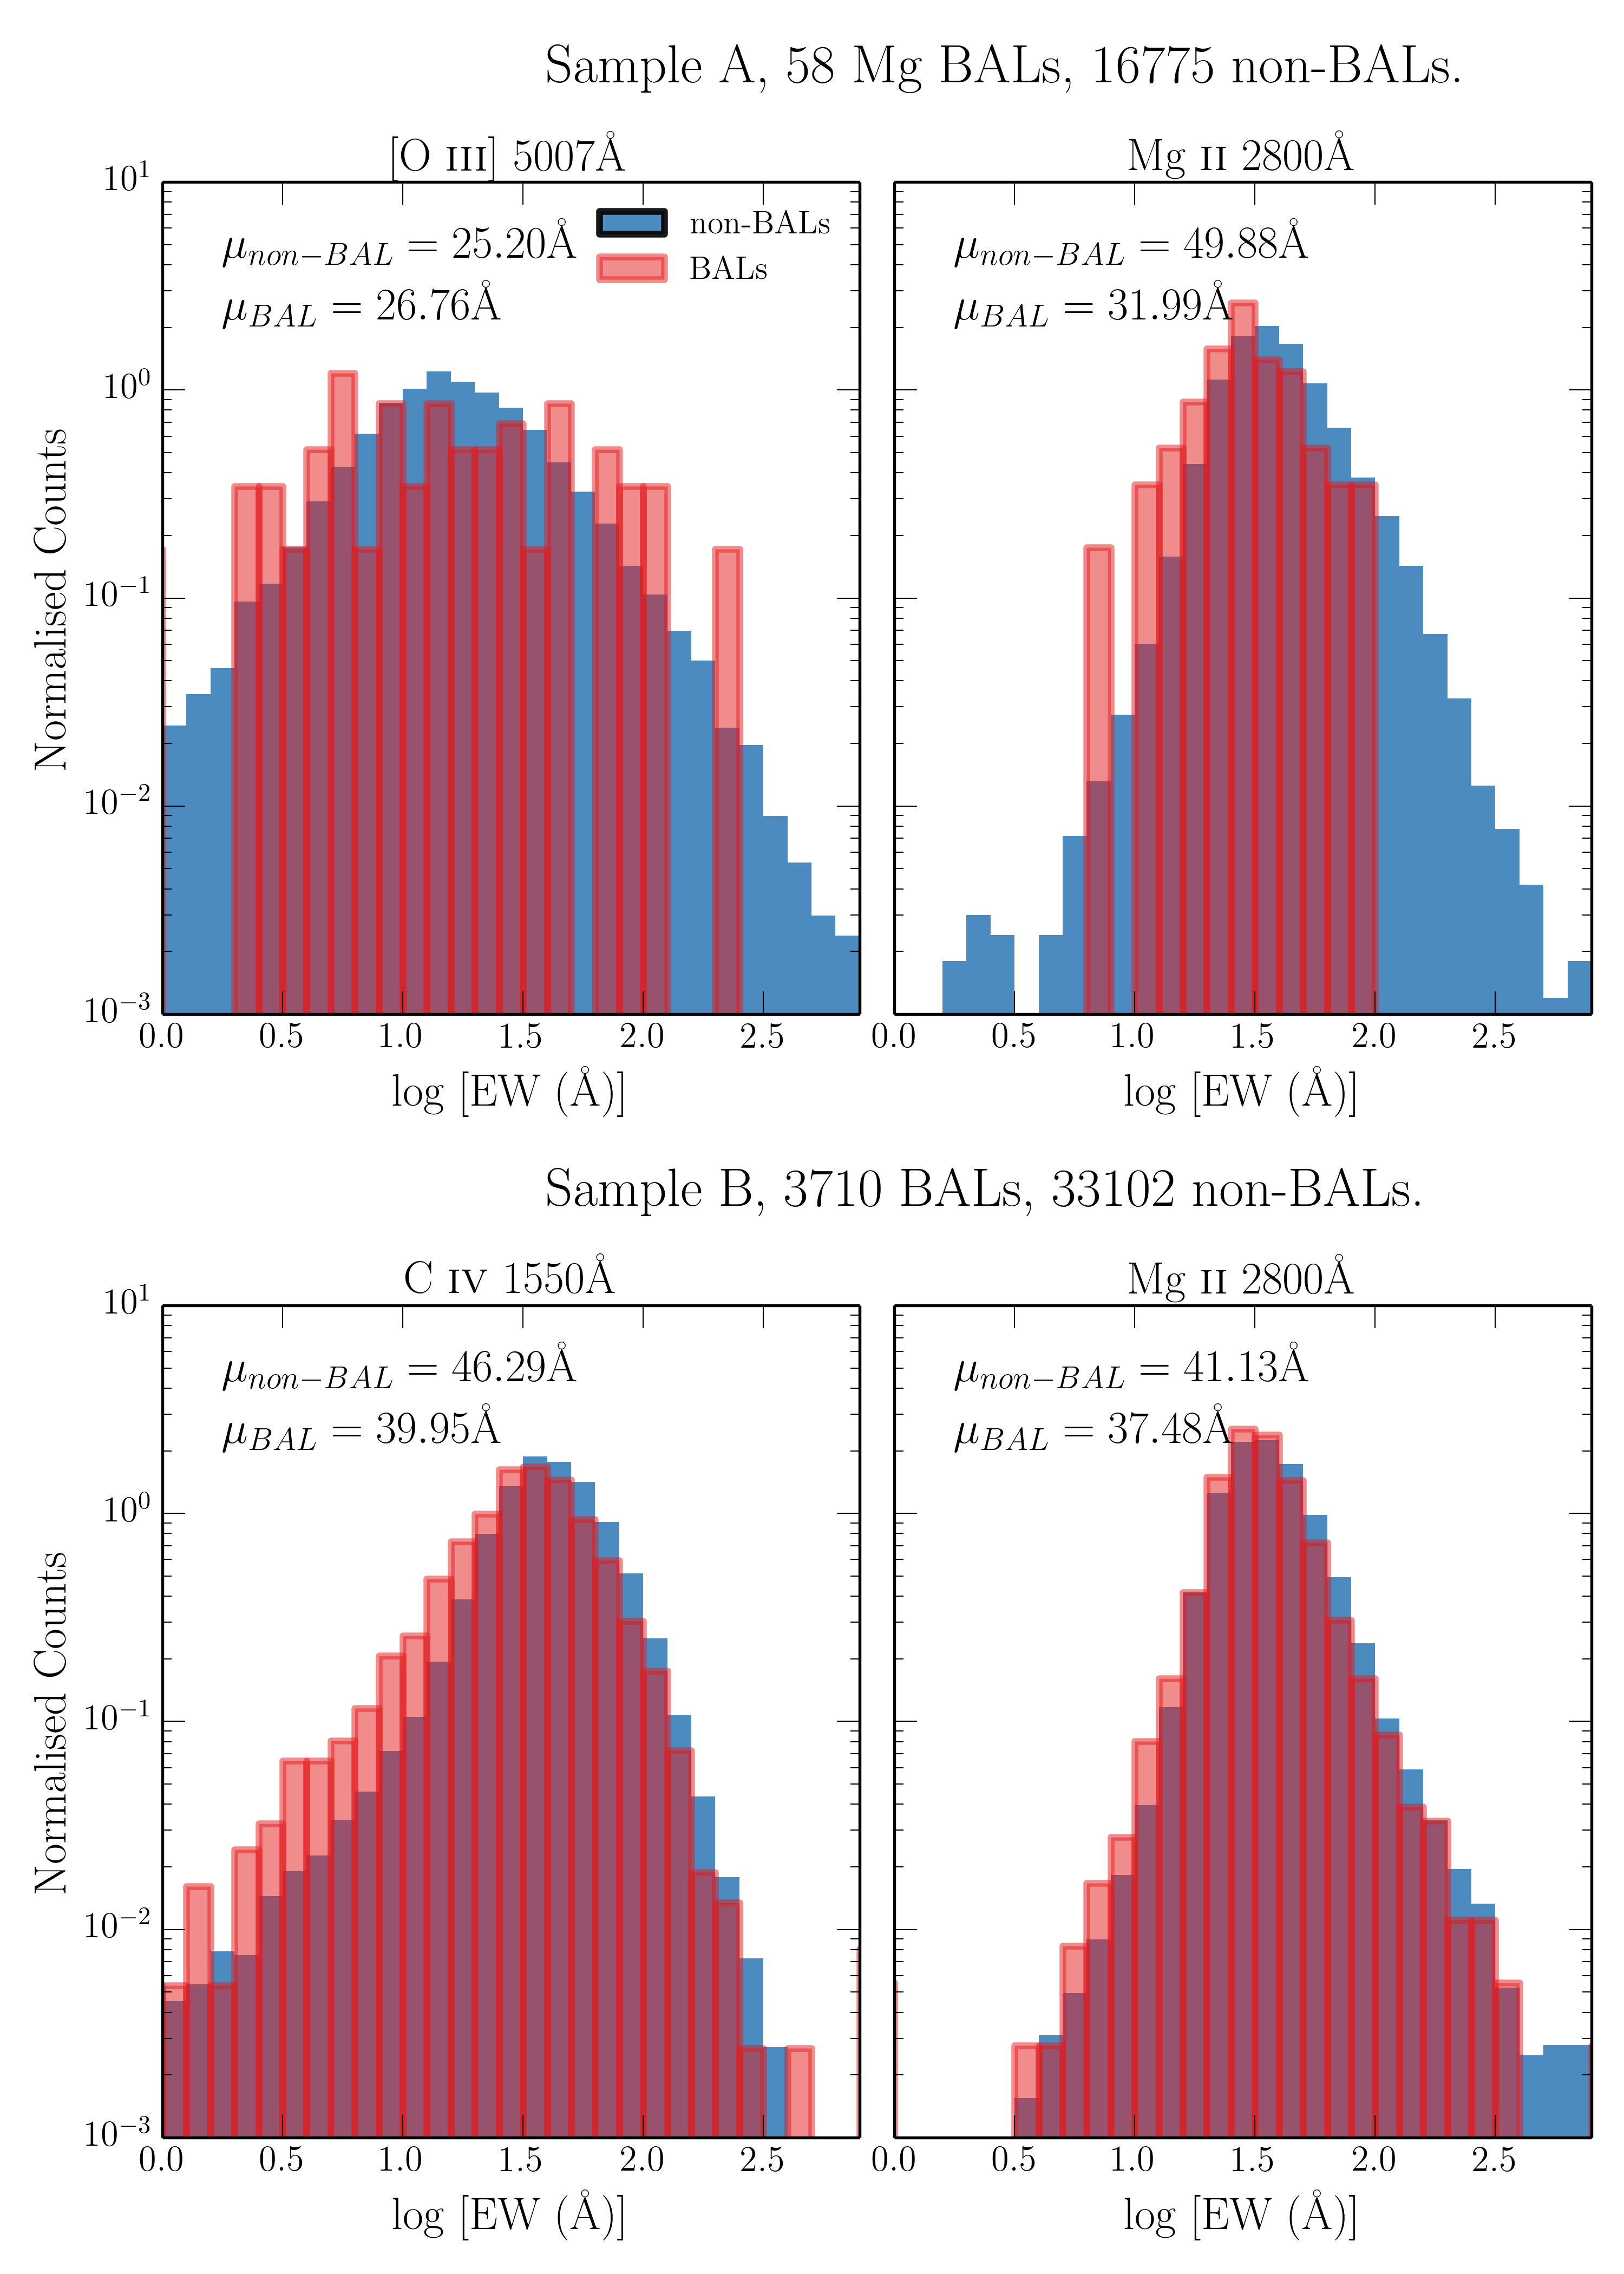
\includegraphics[width=1.0\textwidth]{figures/ewpaper/ew_hist_qsos.png}
\caption
{
Histograms of equivalent widths for three emission lines from the two different samples.
The mean of the BAL and non-BAL quasar distributons are labeled in each case, and
the histograms are normalised so that they integrate to 1.
}
\label{fig:ew_hists}
\end{figure*} %fullpage

The data sample is based upon the
\citet[][hereafter S11]{shen2011} catalog of
105,783 quasars from the The Sloan Digital Sky Survey (SDSS) 
Data Release 7 (DR7). 
As I will use emission line diagnostics in this study,
this sample must be further divided according to which 
emission lines are present in 
the SDSS wavelength range at a given redshift. 
Sample A contains all quasars within the redshift range $0.35<z<0.83$, 
such that the \mgline\ and \oiiifull\ line EWs are both measured, 
and \mg\ BAL identification
is possible.  Sample B contains all quasars within the redshift 
range $1.45<z<2.28$, such that 
the EWs and presence of BAL in \mgline\ and \civline\ are both measurable.
The details of these samples are shown in table 1.
The mass and Eddington fraction measurements from S11 of the two samples,
are shown in Fig.~\ref{fig:bal_scatter}
against the background distribution of all S11 quasars.

S11 are careful to take into account traditional problems with quasar line fitting,
such as narrow line or Fe pseudocontinuum contamination, in their fits to 
emission line profiles and resultant EW measurements. For \mgline\
this includes careful subtraction of the Fe emission using the \cite{vestergaard2001}
templates. This subtraction is not included for \civfull,
as the Fe emission is less prominent and harder to model. This may lead to
a systematic overestimate by $\sim0.05$ dex in the \civ\ line EW. 
The \oiiifull\ line is fitted
with a Gaussian and the flux ratio with the sister component 
of the doublet, \oiiidoublet, is found to agree well with the theoretical
expectation of around 3, implying a reliable subtraction of broad \hb.
To mask out the effects of e.g., absorption, on \civ, S11 ignore 
$3\sigma$ outliers in the fit to the profile. Based on these
considerations, the S11 catalog makes for a reliable set of EW 
measurements. This is especially true when making inferences from 
multiple emission lines, as systematics inherent to individual lines 
or spectral windows are less likely to affect the analysis as a whole.

In attempting to draw broad conclusions about unification models as a whole,
I would ideally construct a large, homogenous dataset of 
{\em HiBAL} and non-BAL quasars, both with \oiiifull\ EWs. Unfortunately,
the wavelength limits of SDSS do not allow this, and only LoBAL quasars have 
both BALs and \ewo\ measurements. One of the problems with
using just LoBAL quasars as tests of unification is that there is evidence 
that they are drawn from a different population than normal quasars. 
Examples include anomalously 
high LoBAL fractions in dust-reddened quasar samples \citep{urrutia2009} 
and infra-red selected samples \citep{dai2012}; 
although see also \cite{lazarova2012}.
% in SDSS by cross-matching the S11 catalog with BALs identified in the HST 
% COS archive.BALs were selected from the COS spectra using the balnicity index, 
% $BI$, defined in equation~??. HST objects were designated as HiBALS 
% by satisfying the condition that $BI>0$ in one of CIV, NV, SiIV.


Fig. 2 shows histograms of a number of different 
emission line properties for samples A and B. 
As discussed by previous authors \cite[e.g.][]{weymann1991}, I find that BAL
and non-BAL quasars really do seem to possess very similar emission line 
properties. The EW is related to the intrinsic, `face-on' equivalent width,
$\ew_*$ by the equation
\begin{equation}
\ew = \ew_* /\epsilon(\theta)
\end{equation}
where $\theta$ is the viewing angle with respect to the symmetry axis 
and $\epsilon(\theta)$ is the `angular emissivity function', which describes 
how the continuum luminosity from the disc varies as a function of viewing angle.
For a foreshortened disc this is simply $\epsilon(\theta) = \cos \theta$. 
Note that this assumes isotropic line emission, but the effect of line
anisotropy is discussed in section~\ref{sec:line_aniso}.

Thus, if BAL quasars are viewed from a larger viewing angle on average then one
would expect them to possess higher EWs, with a broader distribution.
It is already apparent from Fig.~\ref{fig:ew_hists} that the BALQSO distribution mean 
is not significantly higher than the non-BAL quasar
mean -- in fact, in many cases it is lower. This is not expected from a model
in which the continuum is foreshortened and BAL outflows are at all equatorial.
This problem is examined further in section~\ref{sec:mc_angular}. 
First, I will examine the motivations for different forms of \ept\ 
in AGN and quasars.

\section{The Angular Distribution of Emission from an Accretion Disc and Broad-Line Region}
\label{sec:disc_agn}

\noindent 
As introduced in chapter 1, the most widely-used theoretical model for an accretion disc
is the so-called `$\alpha$-disc' model of SS73. 
There are a number of well-documented problems when fitting 
AGN SEDs with SS73 accretion disc models (see section~\ref{sec:disc_continuum}), 
Despite these problems, \cite{capellupo2015} recently had 
some success fitting spectra of AGN when the effects of
GR, mass-loss and comptonisation were included.
In this section, I start by discussing the angular distribution of
emission from an SS73 disc, before exploring opacity and GR 
effects. In order to do so, I use \agn\
\citep{hubeny2000,davishubeny2006,davis2007}. I stress that the 
discussion here is not limited to SS73 discs; the only real condition
for the angular distributions derived here is that the 
disc is geometrically thin and optically thick.

\subsection{Standard Thin Disc Models}

\noindent
Any geometrically thin, optically thick disc will appear
foreshortened and limb darkened (if temperature decreases
with height from the central disc plane). 
Foreshortening is a simple $\cos \theta$ geometric effect, 
where $\theta$ is the inclination with respect to the vertical z axis, which
is perpendicular to the disc plane.
Limb darkening, $\eta(\theta)$, is given by
\begin{equation}
\eta(\theta) = a \left( 1 + b \cos \theta \right),
\end{equation}
where $a$ is a normalisation constant and $b$ governs the strength
of the limb darkening. $b=3/2$, known as the Eddington approximation
tends to given good agreement with solar observations 
\citep[e.g.][]{mihalas}. The two effects can be 
combined to give an angular emissivity function, of
\begin{equation}
\epsilon(\theta) = a \cos \theta \left( 1 + \frac{3}{2} \cos \theta \right).
\end{equation}

\subsection{Including GR and Opacity Effects}

\begin{figure}
\centering
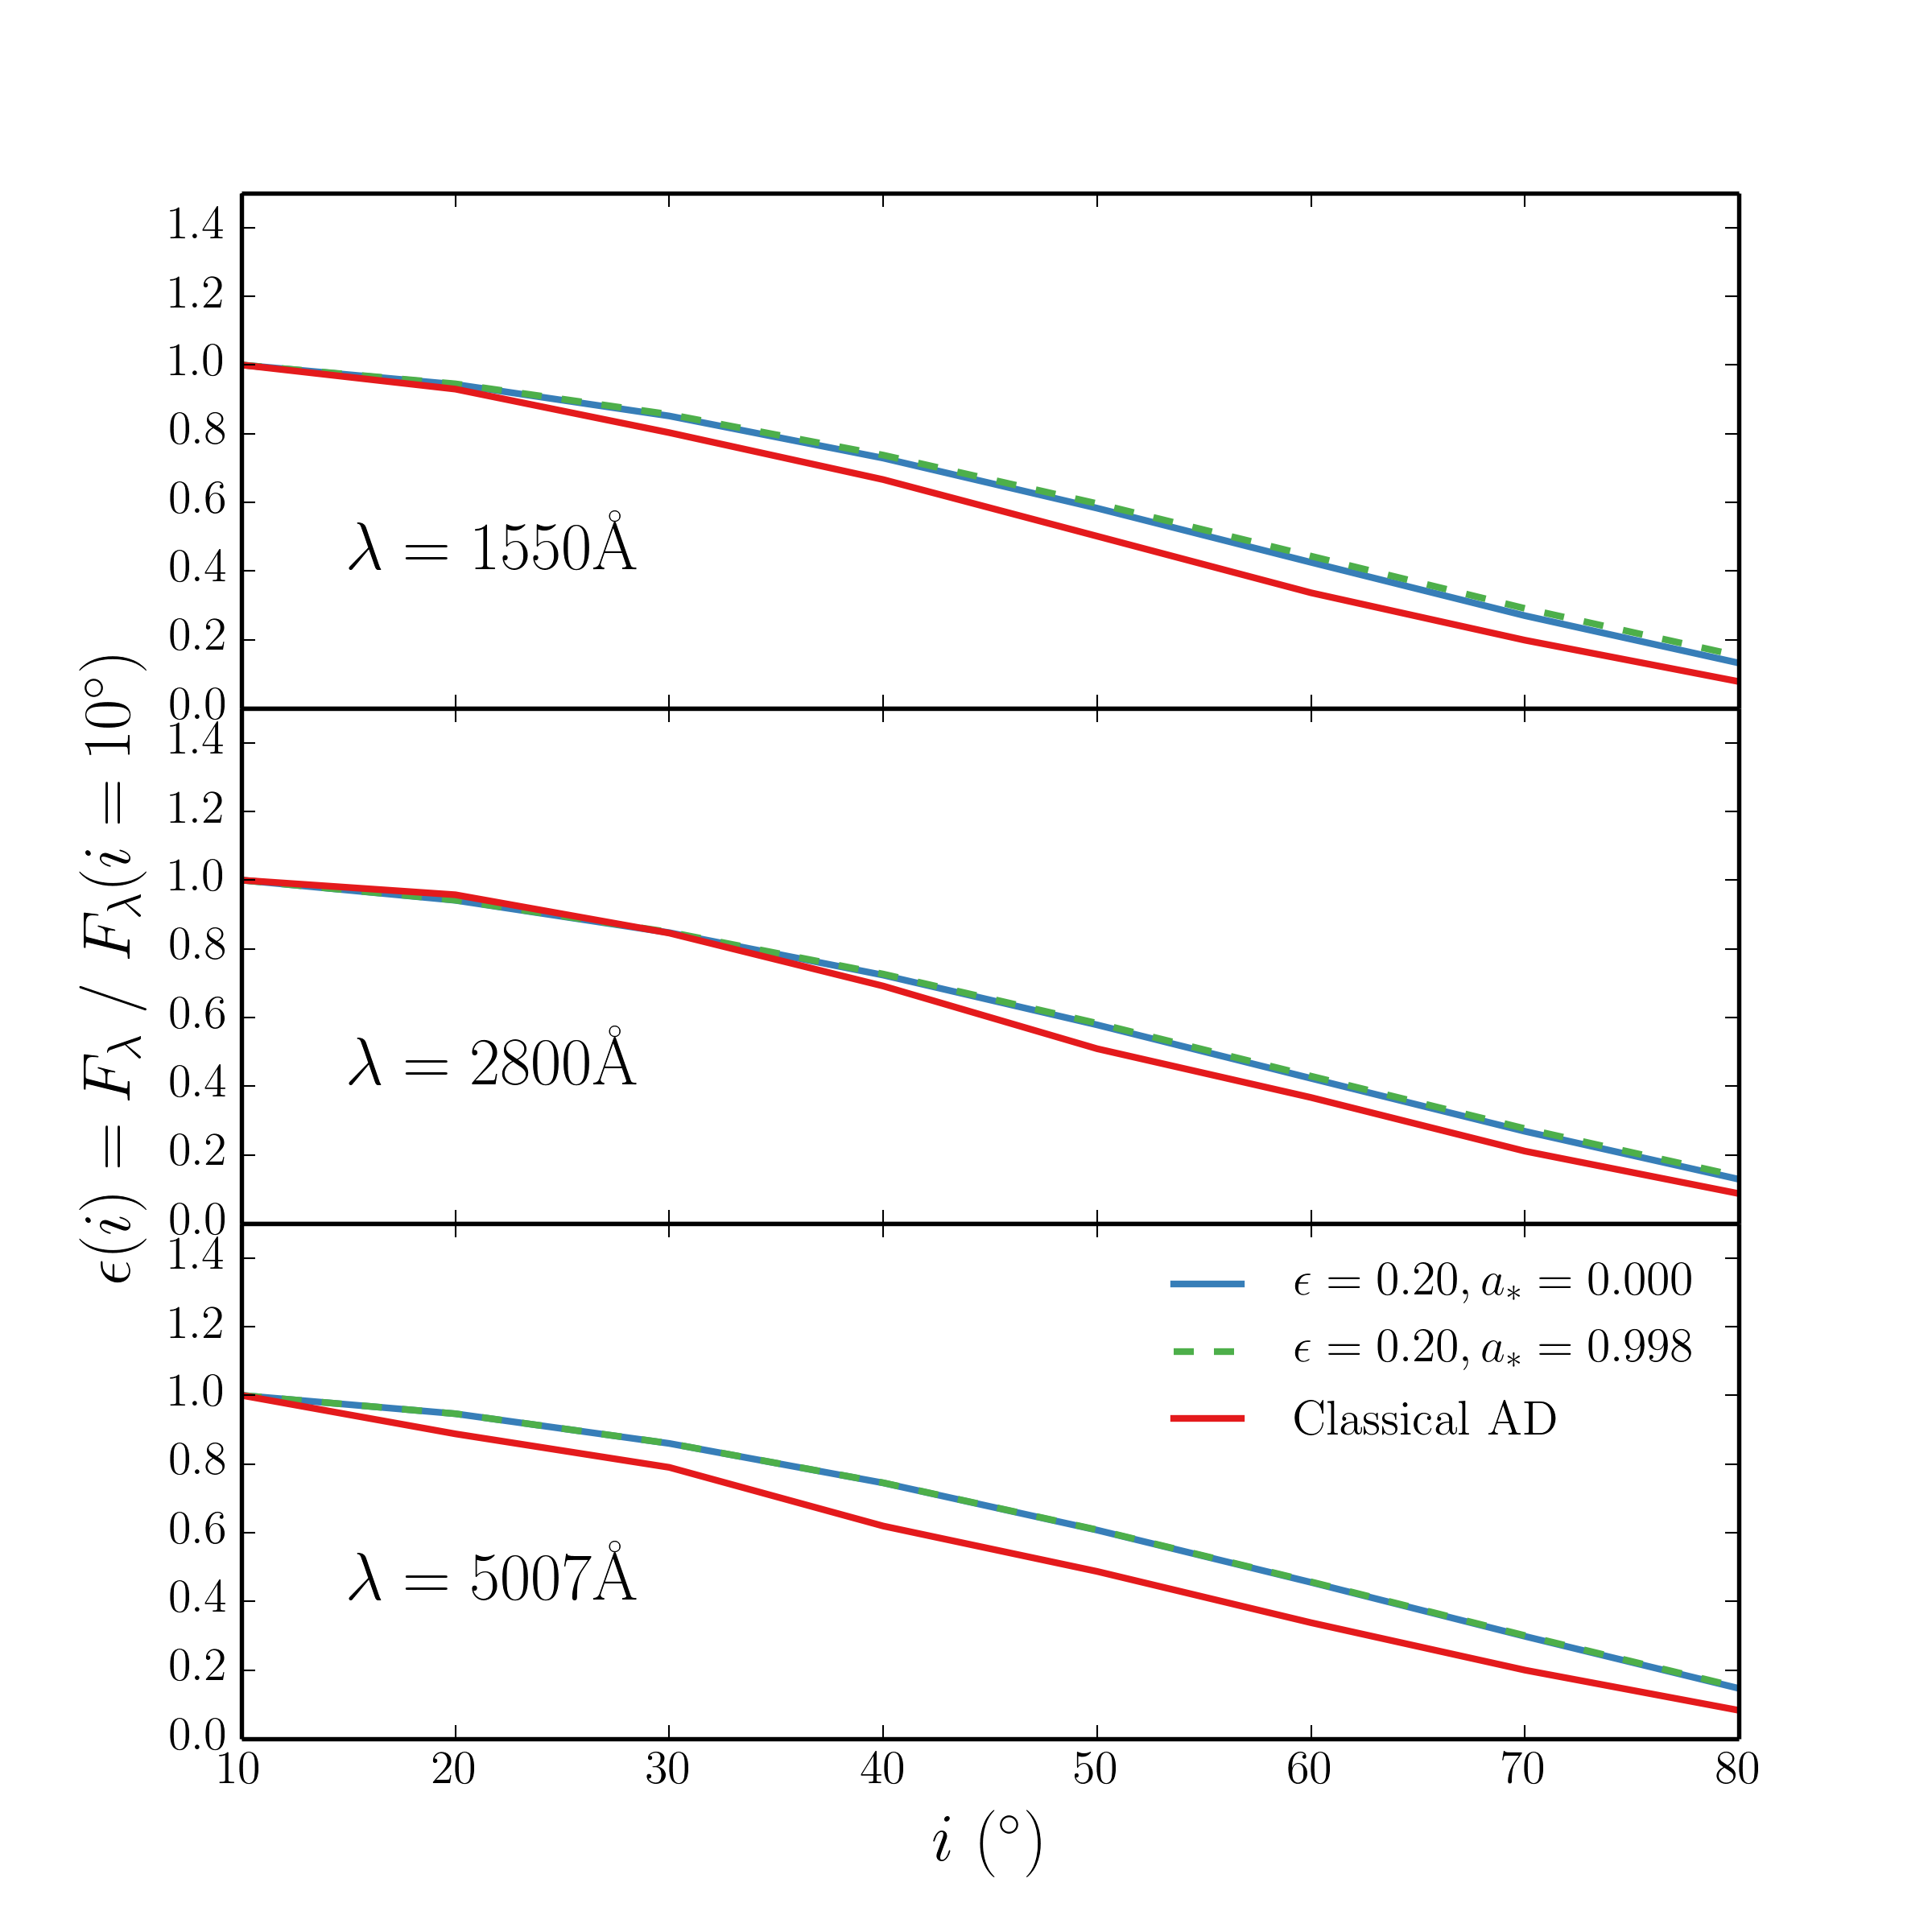
\includegraphics[width=1.0\textwidth]{figures/ewpaper/agnspec.png}
\caption
{
Monochromatic continuum luminosities from AGNSPEC and classical thin disc
models.
}
\label{fig:agnspec_disc}
\end{figure} 


\noindent
In reality, limb darkening is not frequency independent and 
depends on the bound-free and bound-bound opacities in the disc.
In addition, it has been shown that GR can `isotropize' the radiation
field in XRBs \citep{zhang1997,munozdarias2013}, in some cases overcoming
foreshortening effects. To assess the impact of GR and disc opacities
on \ept, I use \agn\ models, which conducts a stellar atmosphere calculation
to obtain the SED from a series of annuli, before using the \kerrtrans\ code 
to calculate the emergent SED by ray-tracing along Kerr geodesics.
Fig.~\ref{fig:agnspec_disc} shows \ept\ as a function of 
$\theta$ for \agn\ models for minimally and maximally spinning BHs,
compared to foreshortened and limb-darkened predictions for SS73 models.
Although the continuum is significantly more isotropic at $500$\AA,
there is very little effect redward of around $1000$\AA, which is the relevant
region of \ept\ for \oiiifull, \civline\ and \mgline . 
In fact, using the foreshortened estimate is 
the conservative approach in these regimes. I will thus adopt \ept$=\cos \theta$
for the remainder of this work.


% Including GR, Comptonisation and Opacity Effects

% \subsection{Alternative Continuum Models: Irradiation and Truncated Discs}

% Alternative Models exist...


% \subsection{Angular Distribution of Line Emission}

% Lines can be classified according to whether they violate quantum selection rules.
% In order of decreasing oscillator strength, they comprise
% dipole permitted transitions, such as \civline\ and \hb, 
% semi-forbidden or intercombination
% lines such as \ciiiline, and forbidden lines such as \oiiifull.
% As the optical depth in a line is proportional to the oscillator strength,
% we can see that we should expect lines such as \oiiifull\ to be optically
% thin, whereas dipole transitions may be subject to local line
% opacity effects. It is worth noting, of course, that all lines can be absorbed by 
% continuum processes. Ignoring the effect of obscuration, we thus expect all 
% forbidden lines to be isotropic (i.e. \eptl$={\rm constant}$. 
% But what about permitted lines? What is their expected angular distribution
% of emission

\section{Predicted EW Distributions Compared to Observations}
\label{sec:mc_angular}

\subsection{Fitting the Quasar Distribution}
\label{sec:fitting}

\citet[][hereafter R11]{risaliti2011} analysed the \ewo\ 
distribution of 6029 quasars in SDSS DR5. They demonstrated
that a foreshortened disc and isotropic \oiiifull\ line produces
a high EW tail to the distribution with a characteristic 
slope of $\Gamma_{EW}=-3.5$. In order to first reproduce their
result and discuss its implications, I have 
created a sample according to their selection
criteria. The criteria are that the object in question lies in the redshift
range 0.01 to 0.8, have an absolute magnitude $M_i>22$, an 
apparent magnitude $m_i>19.1$, and signal to noise per pixel of greater
than 5. Using the updated SDSS quasar sample of S11, this defines
a sample of 14,424 quasars.

To fit the distribution, I conduct the following procedure,
which is similar to the method R11 use to demonstrate that the power
law tail is expected.
\begin{enumerate}
	\setlength\itemsep{1em}
	\item A set of isotropic angles is chosen such that 
	$P(\theta)\propto d\Omega(\theta)$. 
	If $\theta<\theta_{1}$ then the fake object is designated as unobscured, 
	and otherwise the object is ignored. 
	\item To be included in the sample, the object also has to 
	survive a selection test
	to simulate the distribution of angles in a flux-limited sample.
	This is done by drawing a random sample from the real quasar sample, 
	and calculating a `doubly observed continuum flux', $F_O$ at $5100\AA$ 
	(rest frame), such that $F_O = F_{5100}~\epsilon(\theta)$. The flux limit
	is set at $5\times10^{-13}$~erg~s$^{-1}$~cm$^{-1}$~\AA$^{-1}$, but the results
	are fairly insensitive to the limit chosen.
	\item For each mock sample, an EW$_*$ is drawn from an intrinsic 
	(i.e. `face-on') EW distribution for quasars. This is assumed to be a
	Gaussian distribution. The mean, $\mu_*$, and width, $\sigma_*$, of this Gaussian
	can either be set arbitrarily -- for example, to demonstrate trends
	in mock data -- or obtained from a $\chi^2$ fit to the observed EW
	distribution.
	\item A mock EW is estimated such that $\ew = \ew_* / \epsilon(\theta)$,
	and this process is repeated to build up a mock sample of $10^6$ objects.
\end{enumerate}
The result of this numerical experiment is, as found by R11, a distribution
with a high EW tail of slope $-3.5$. I can now vary the maximum angle, $\theta_1$,
and examine how this tail changes. Mock data for a series
of maximum angles is shown in Fig.~\ref{fig:cutoff}, for two different intrinsic 
Gaussians. The power law behaviour is only seen when the maximum angle is
sufficiently large, and a rapid decay in the distribution is observed
at a characteristic EW related to both the width and mean of the
intrinsic distribution as well as the cosine of the maximum angle.
The top panel has $\mu_*$ and $\sigma_*$ of the R11 Model 1, 
whereas the bottom panel shows a narrower distribution to illustrate the 
earlier onset of the high EW cutoff. In principle, this cutoff could
be used to infer information about the viewing angle distribution
of quasars.

\begin{figure}
\centering
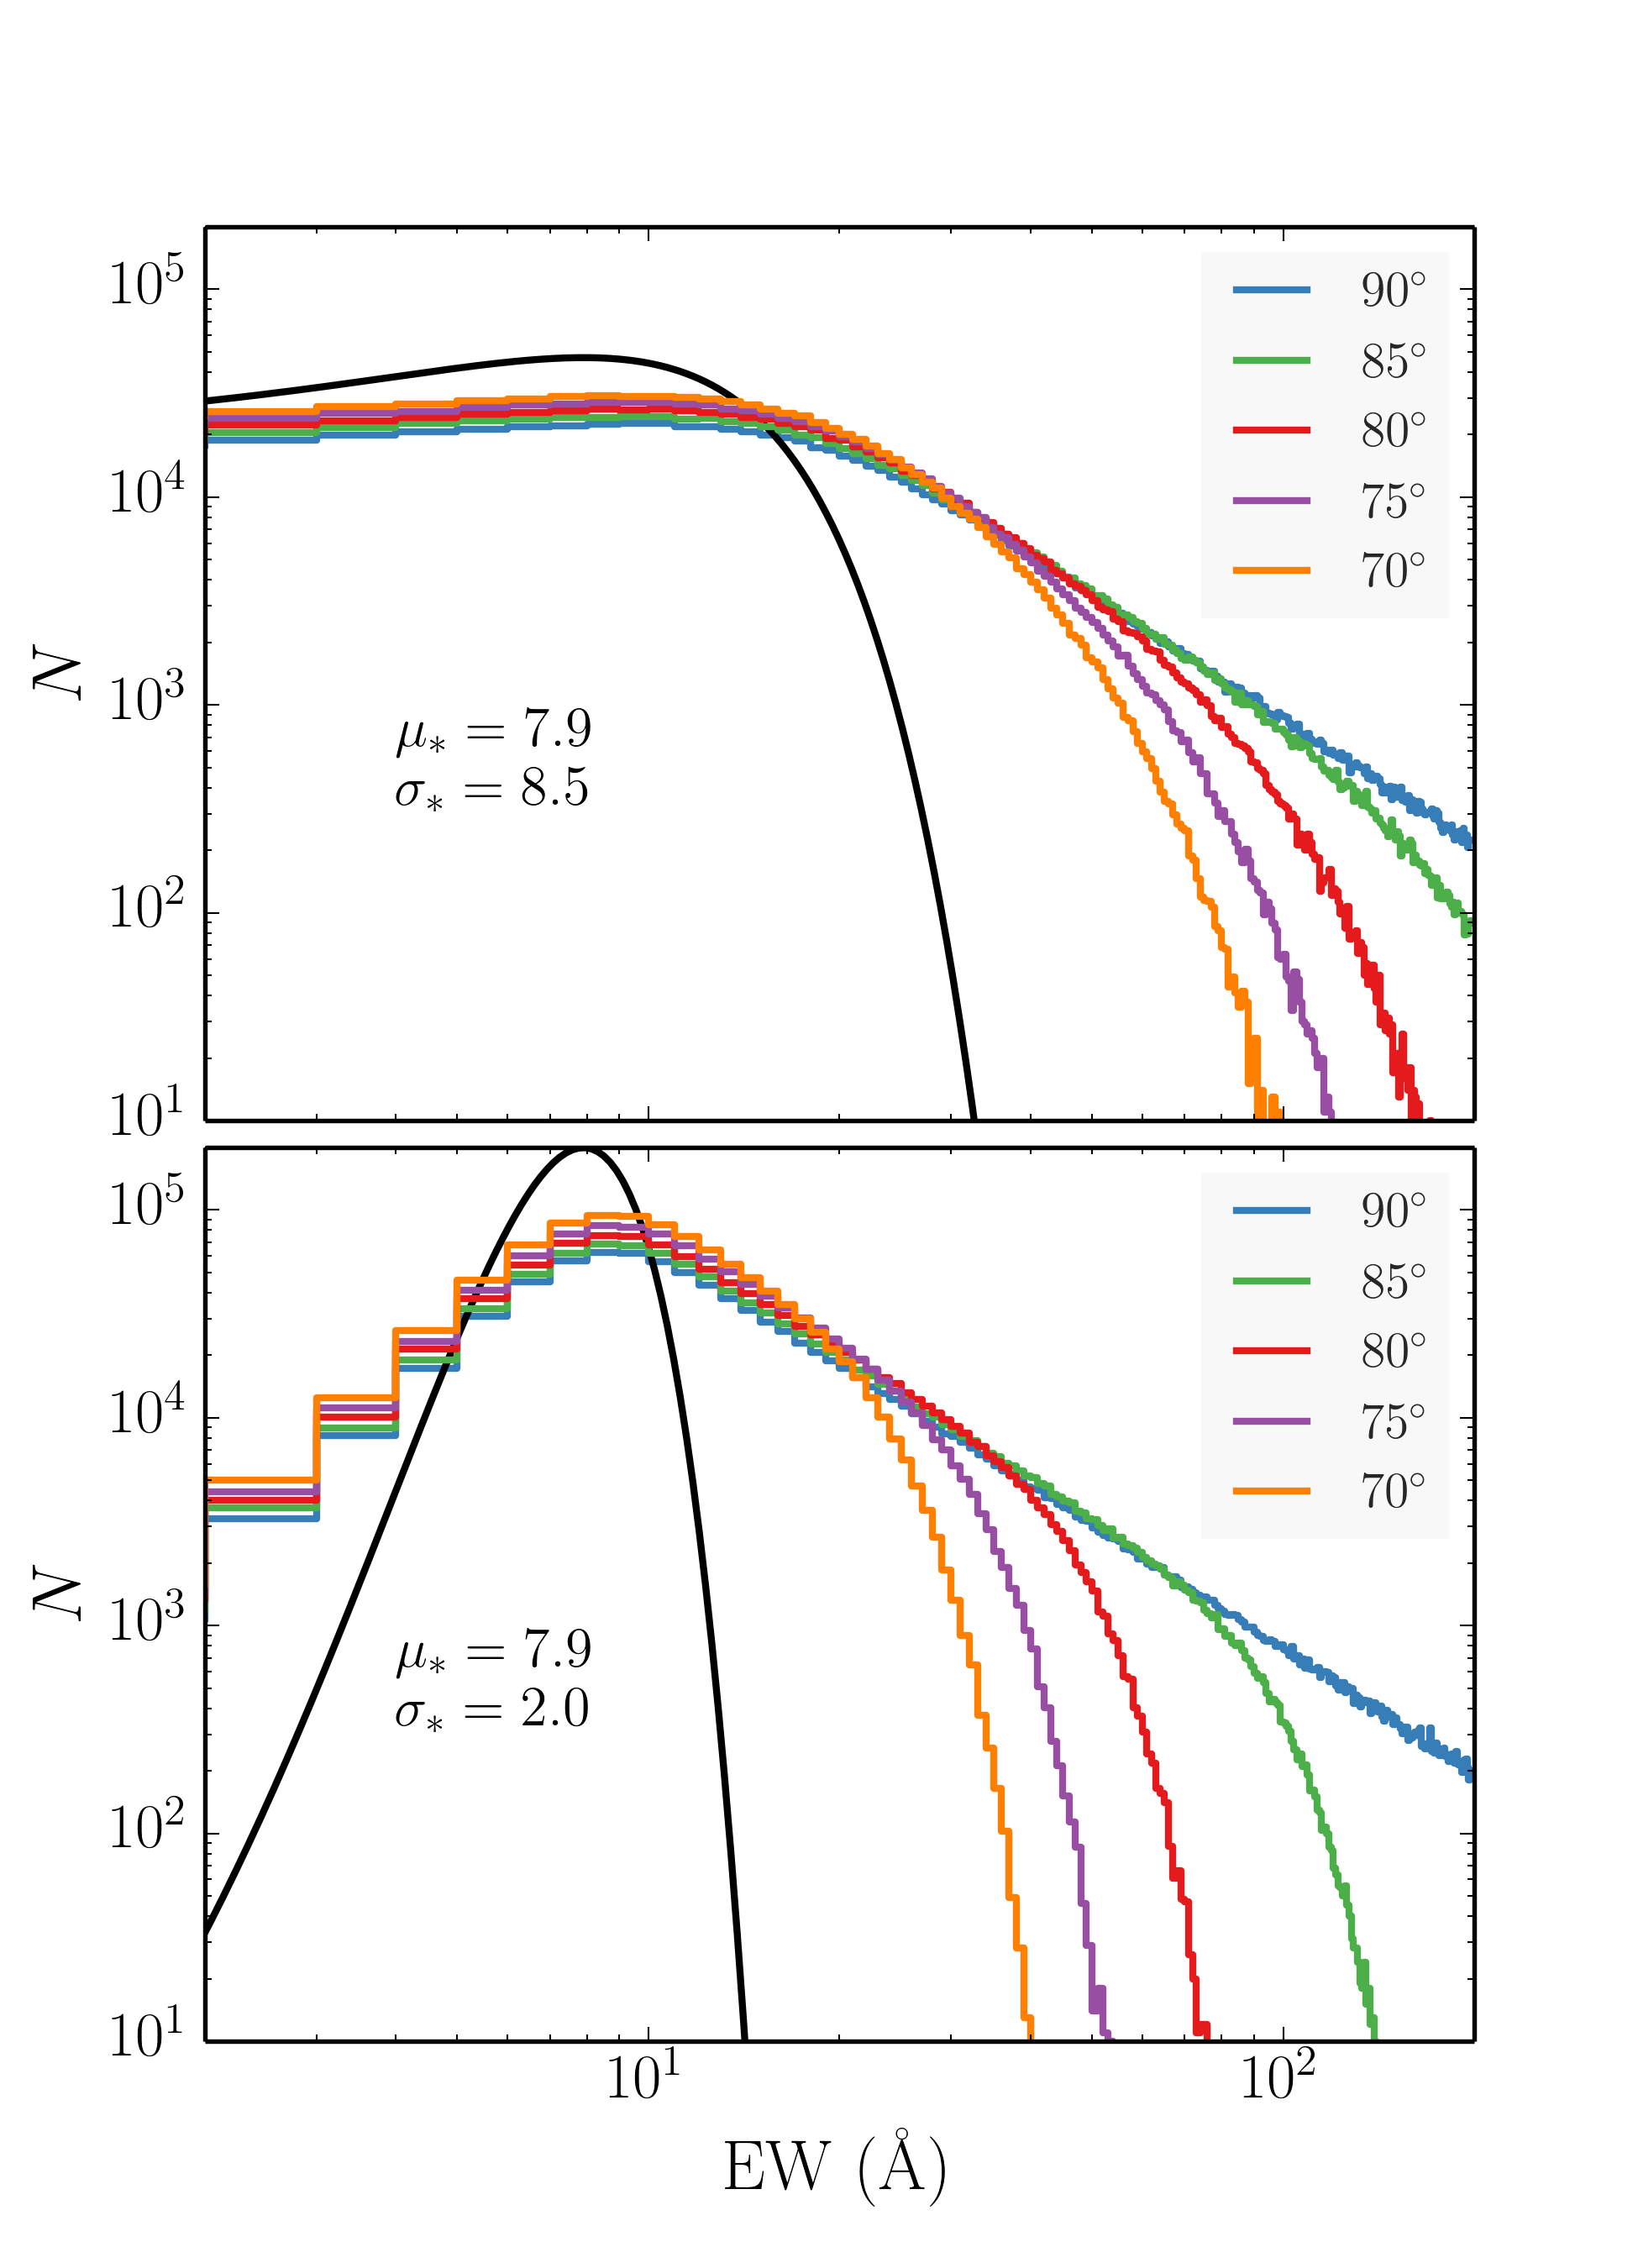
\includegraphics[width=1.0\textwidth]{figures/ewpaper/cutoff.png}
\caption
{
Theoretical EW distributions from the numerical experiment 
described in section~\ref{sec:fitting} for a few different 
maximum angles. The results in the top panel use the same intrinsic
distribution as Model 1 from R11 (shown in black), 
whereas the bottom panel shows the distributions 
obtained from a narrower intrinsic Gaussian. By the time the maximum
angle is limited to around $70^\circ$ the cutoff is
clear even at moderate values of EW.
}
\label{fig:cutoff}
\end{figure}

Fig.~\ref{fig:chi2} shows the result of a $\chi^2$ minimization fit 
to the R11 sample. The best fit is achieved with a maximum angle of 
$\theta_{1}=84^\circ$ and a narrower intrinsic distribution
than model 1 of R11. The run of reduced $\chi^2$ with maximum angle
is shown in Fig.~\ref{fig:chi2_curve}, where the choice for $\mu_*$
and $\sigma_*$ is left free in each case. 
Maximum angles below $\sim80^\circ$ are strongly disfavoured
by this model. I adopt linear binning to facilitate easy comparison 
with R11, and only fit up $\ew=100$\AA\
due to poor statistics above that limit. This 
makes inferring any information about a potential high EW cutoff 
difficult as a more complete sample at high EW is required. 

\begin{figure}
\centering
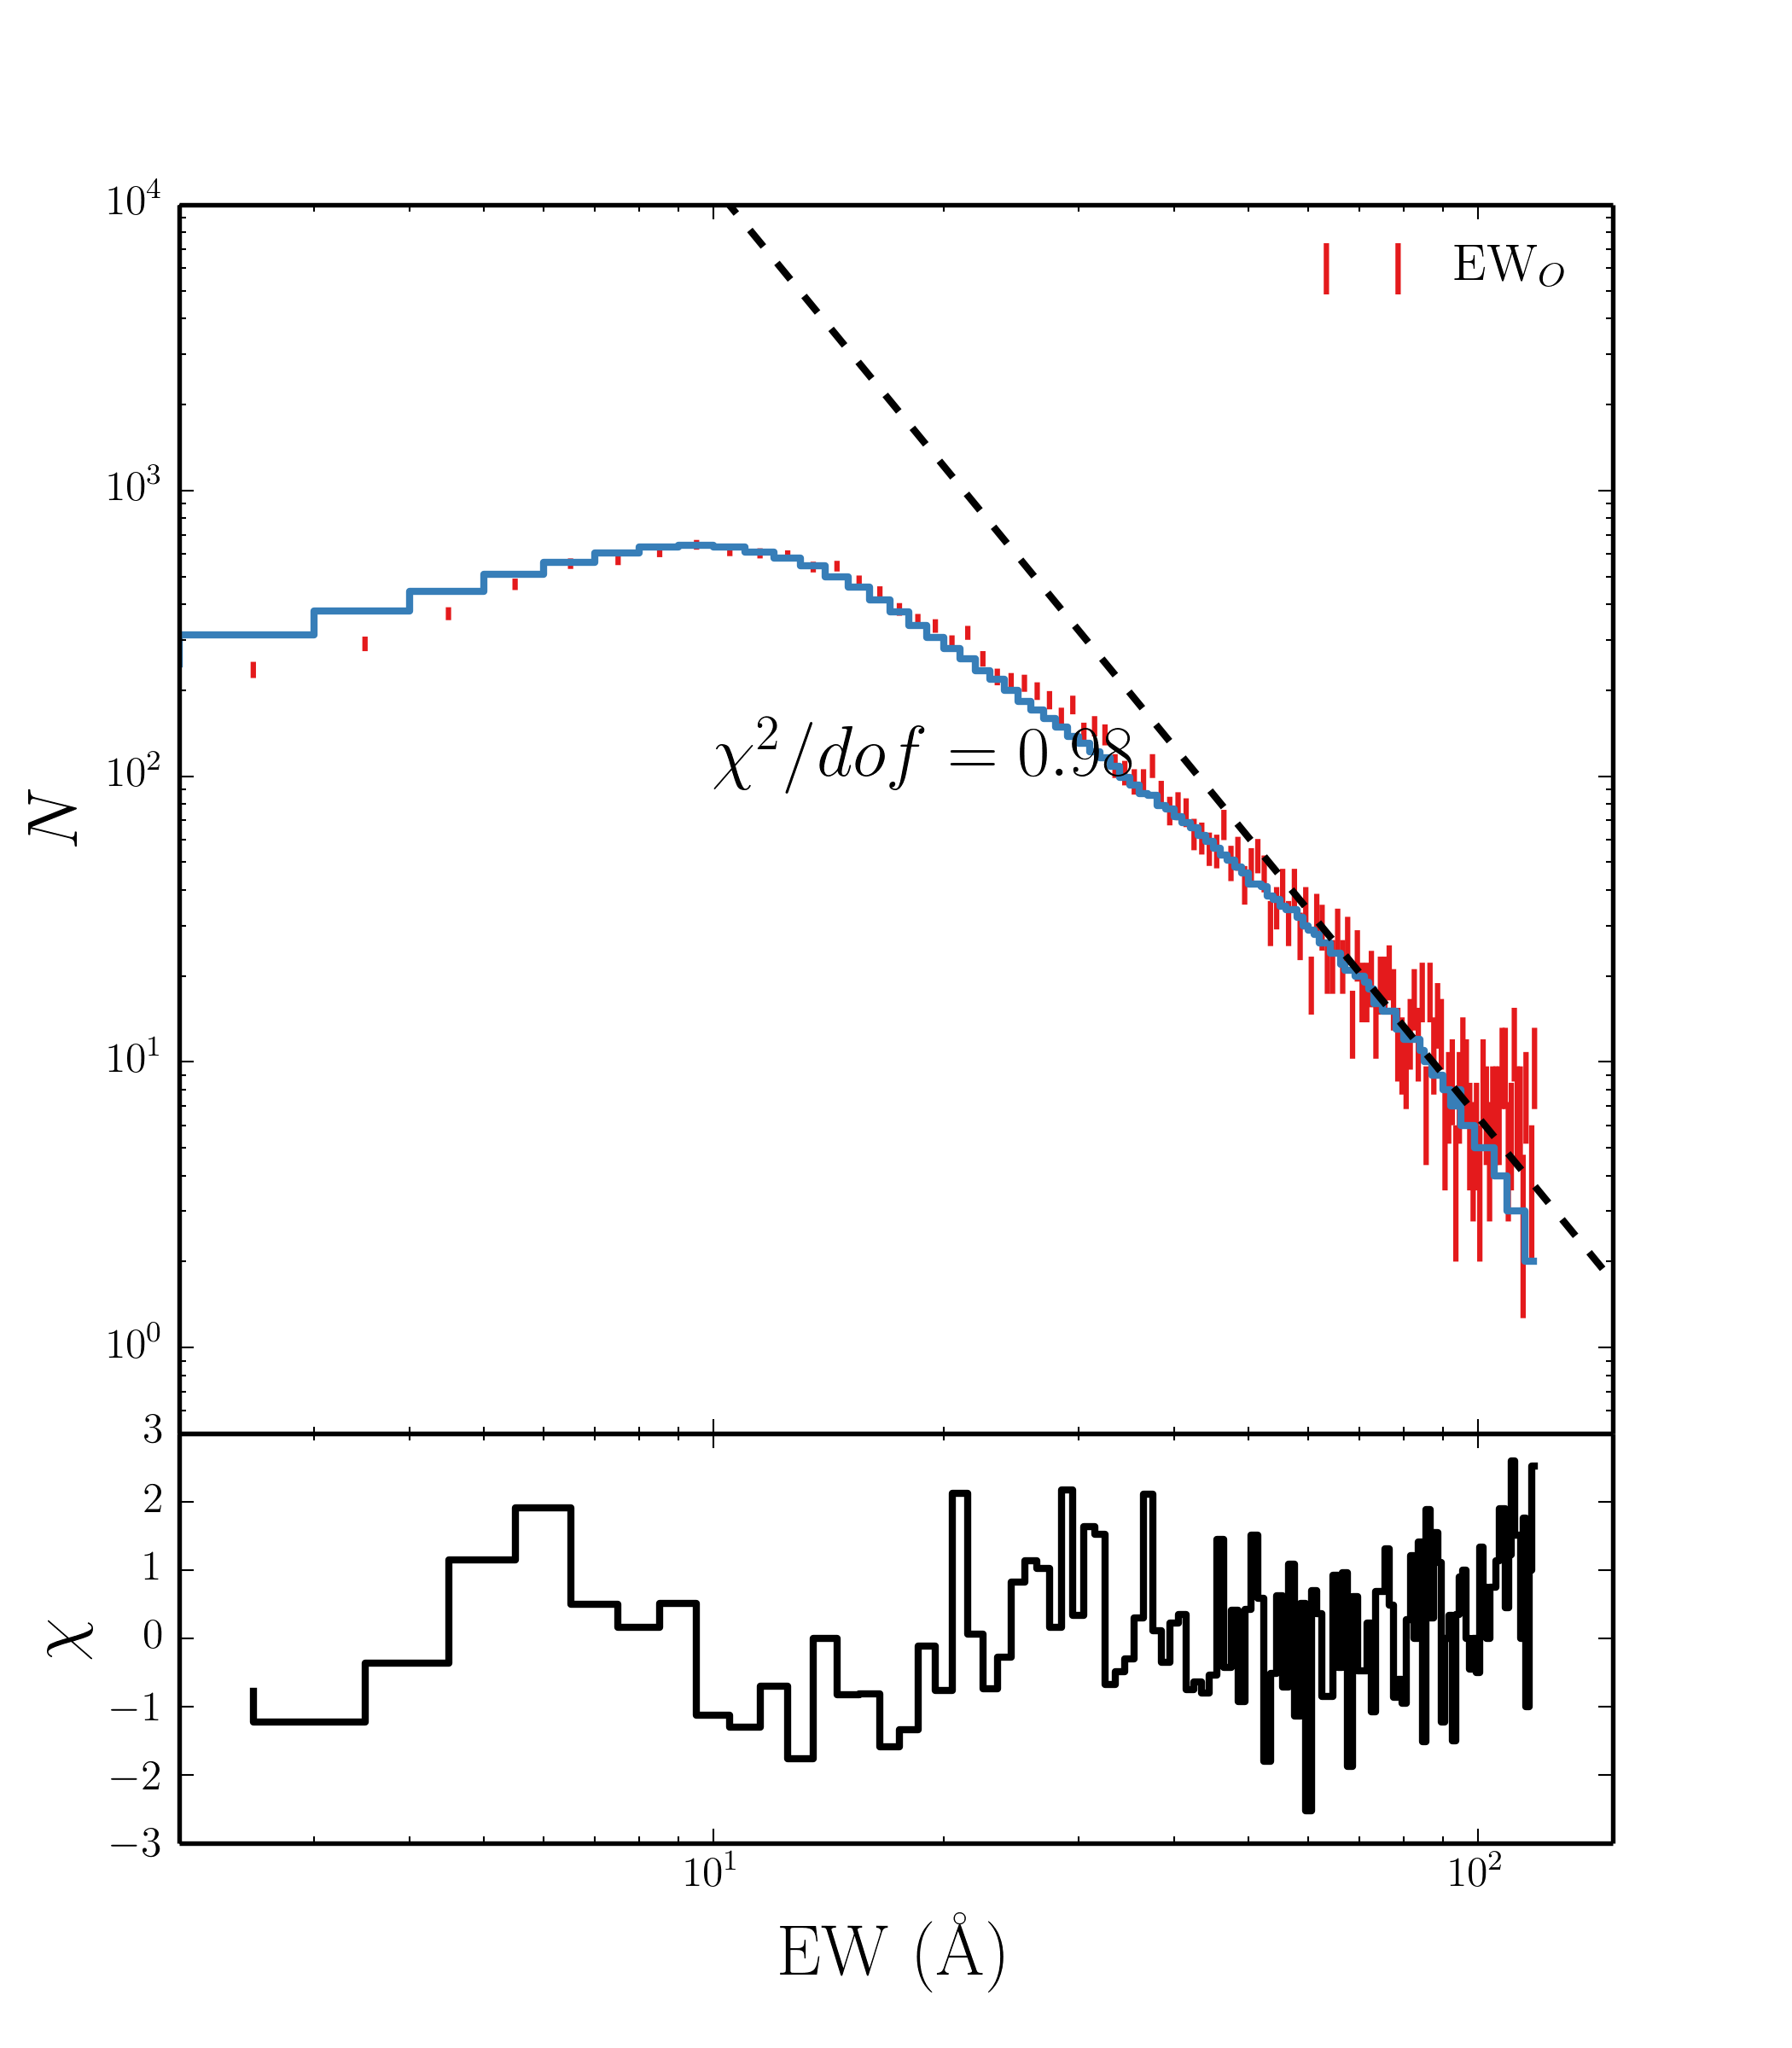
\includegraphics[width=1.0\textwidth]{figures/ewpaper/log_quasar_fit.png}
\caption
{
The EW distribution of quasars in the R11 sample (black points), 
with $\sqrt{N}$ errorbars, and the best fit model with a maximum 
viewing angle of $84^\circ$. The intrinsic Gaussian distribution
is shown with a dotted line. 
}
\label{fig:chi2}
\end{figure}

\begin{figure}
\centering
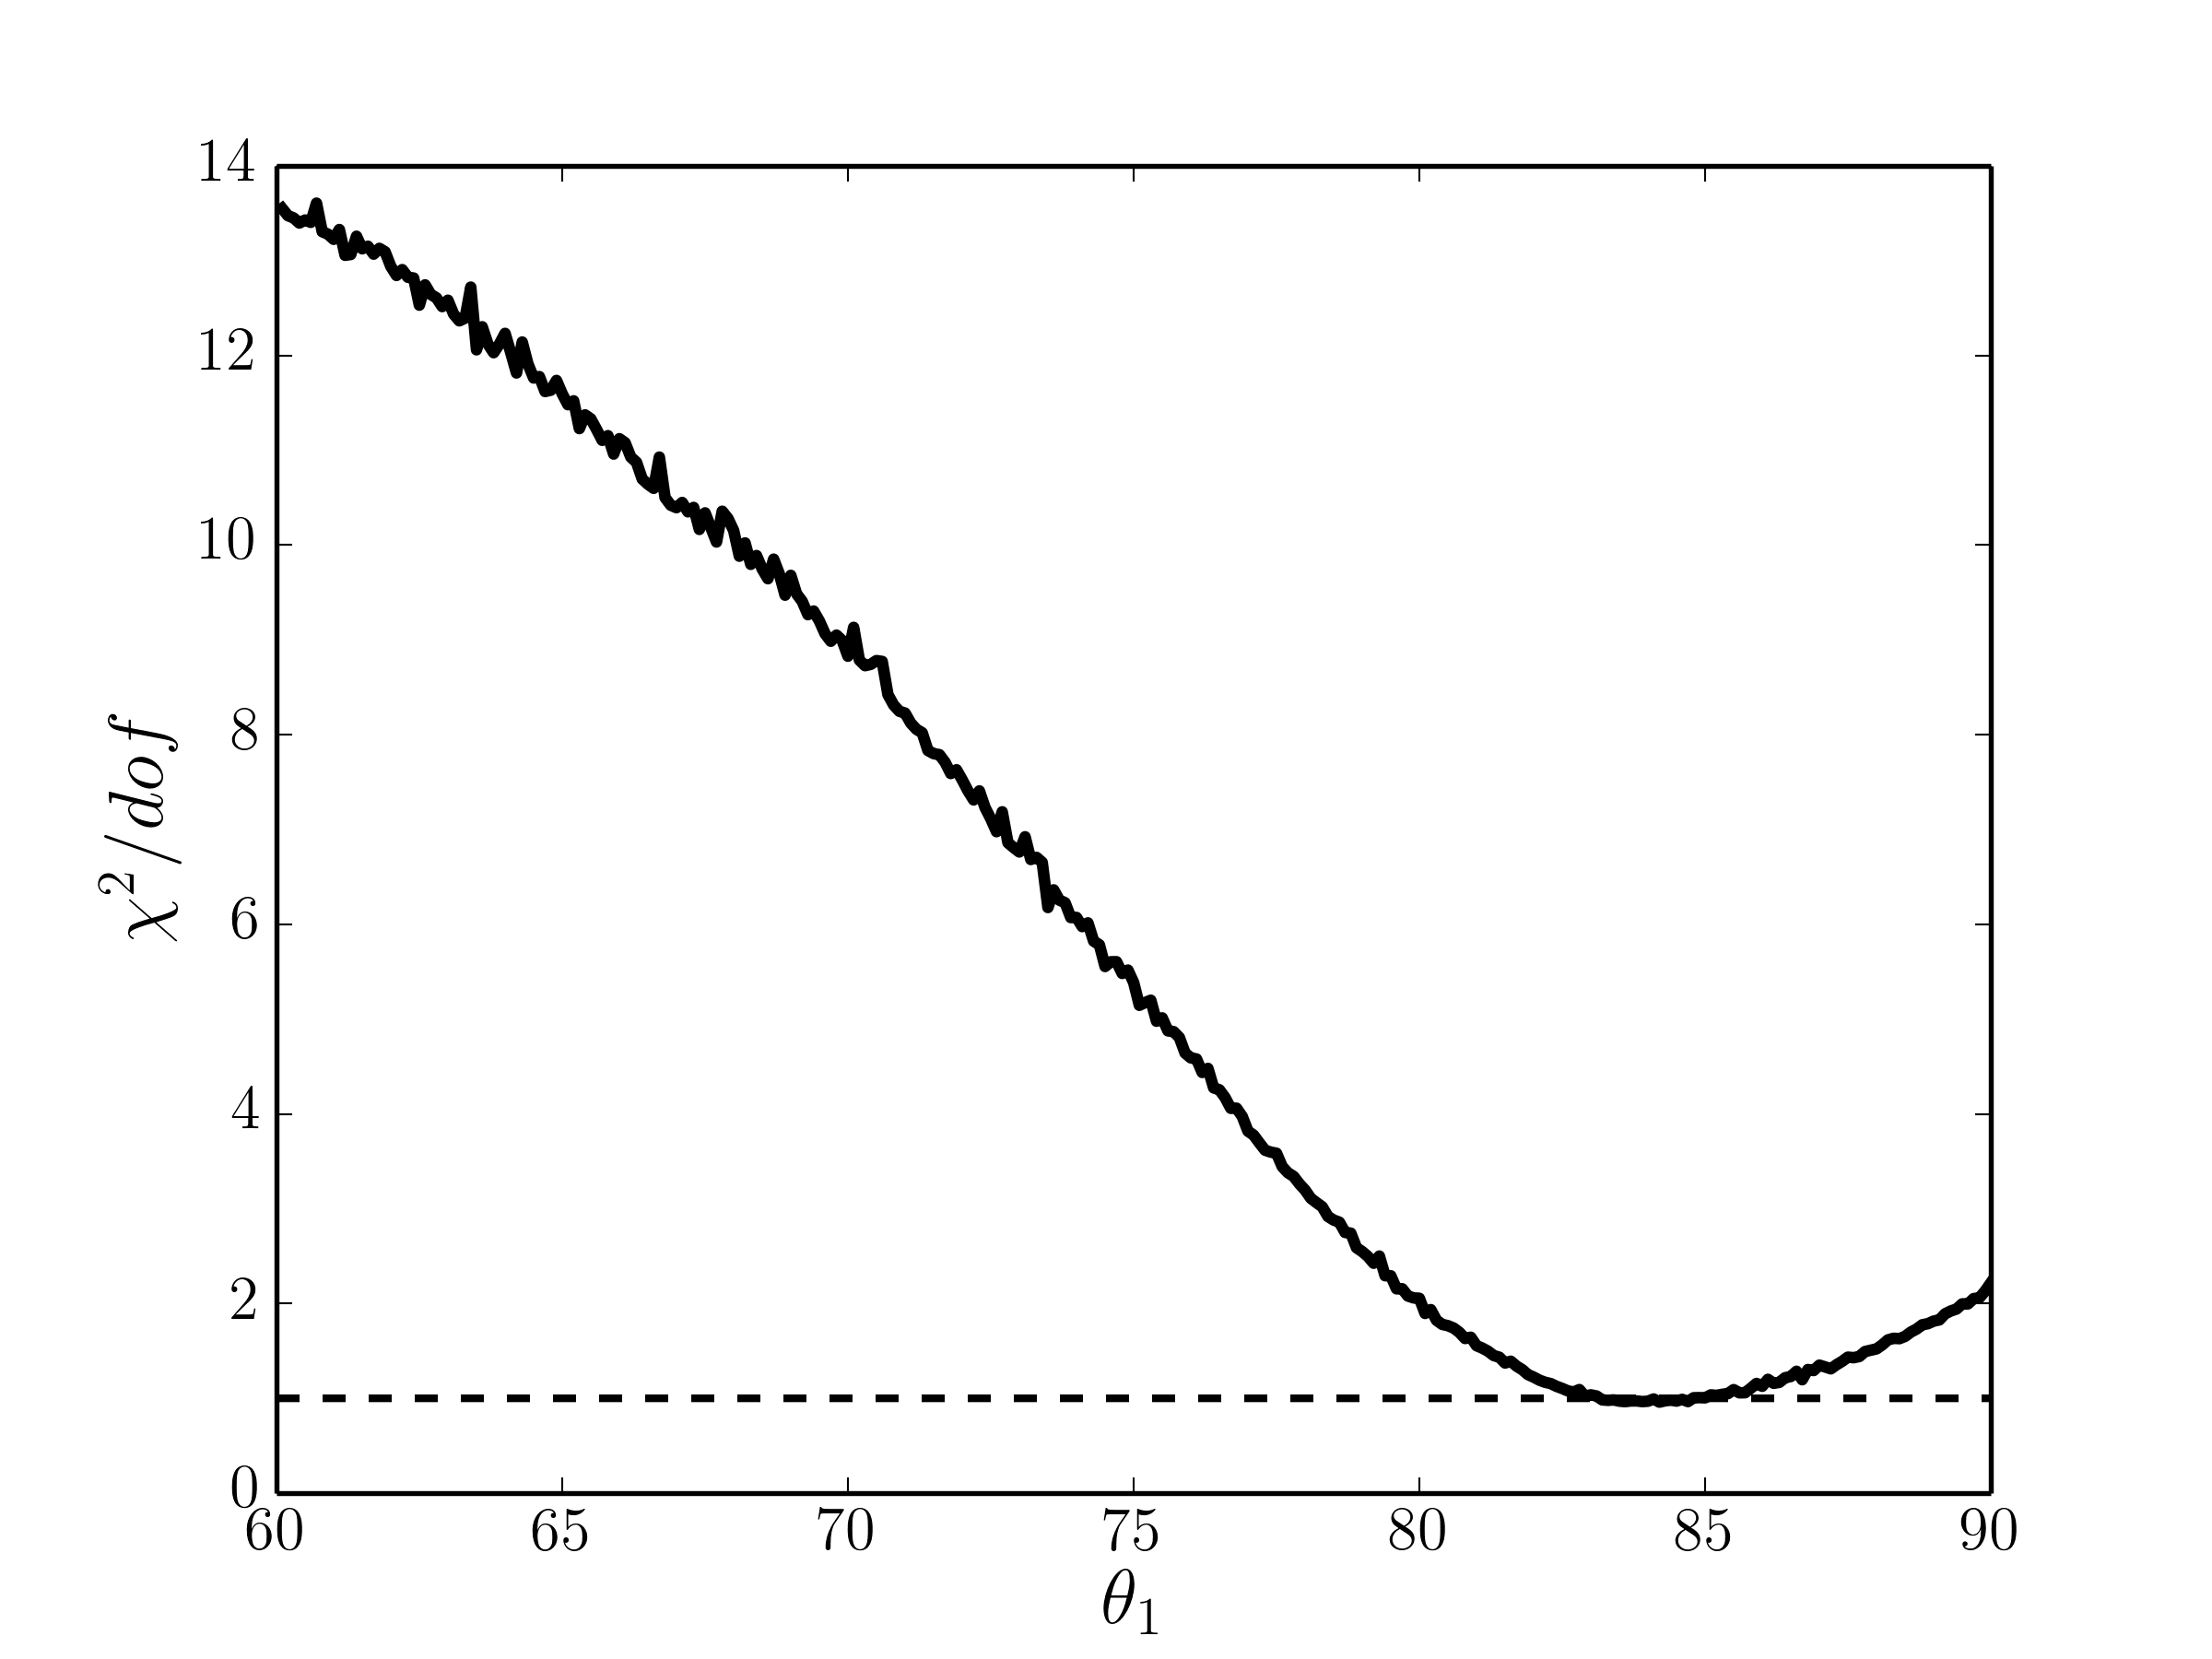
\includegraphics[width=0.8\textwidth]{figures/ewpaper/chi2_o3.png}
\caption
{
$\chi^2/dof$ as a function of maximum angle, $\theta_1$, calculated in
steps of $0.1^\circ$. The choice for $\mu_*$ and $\sigma_*$ is 
left free in each case.
}
\label{fig:chi2_curve}
\end{figure}

\subsection{Comparing non-BAL and LoBAL Distributions: Sample A}
\label{sec:bal_v_nonbal}

\begin{figure}
\centering
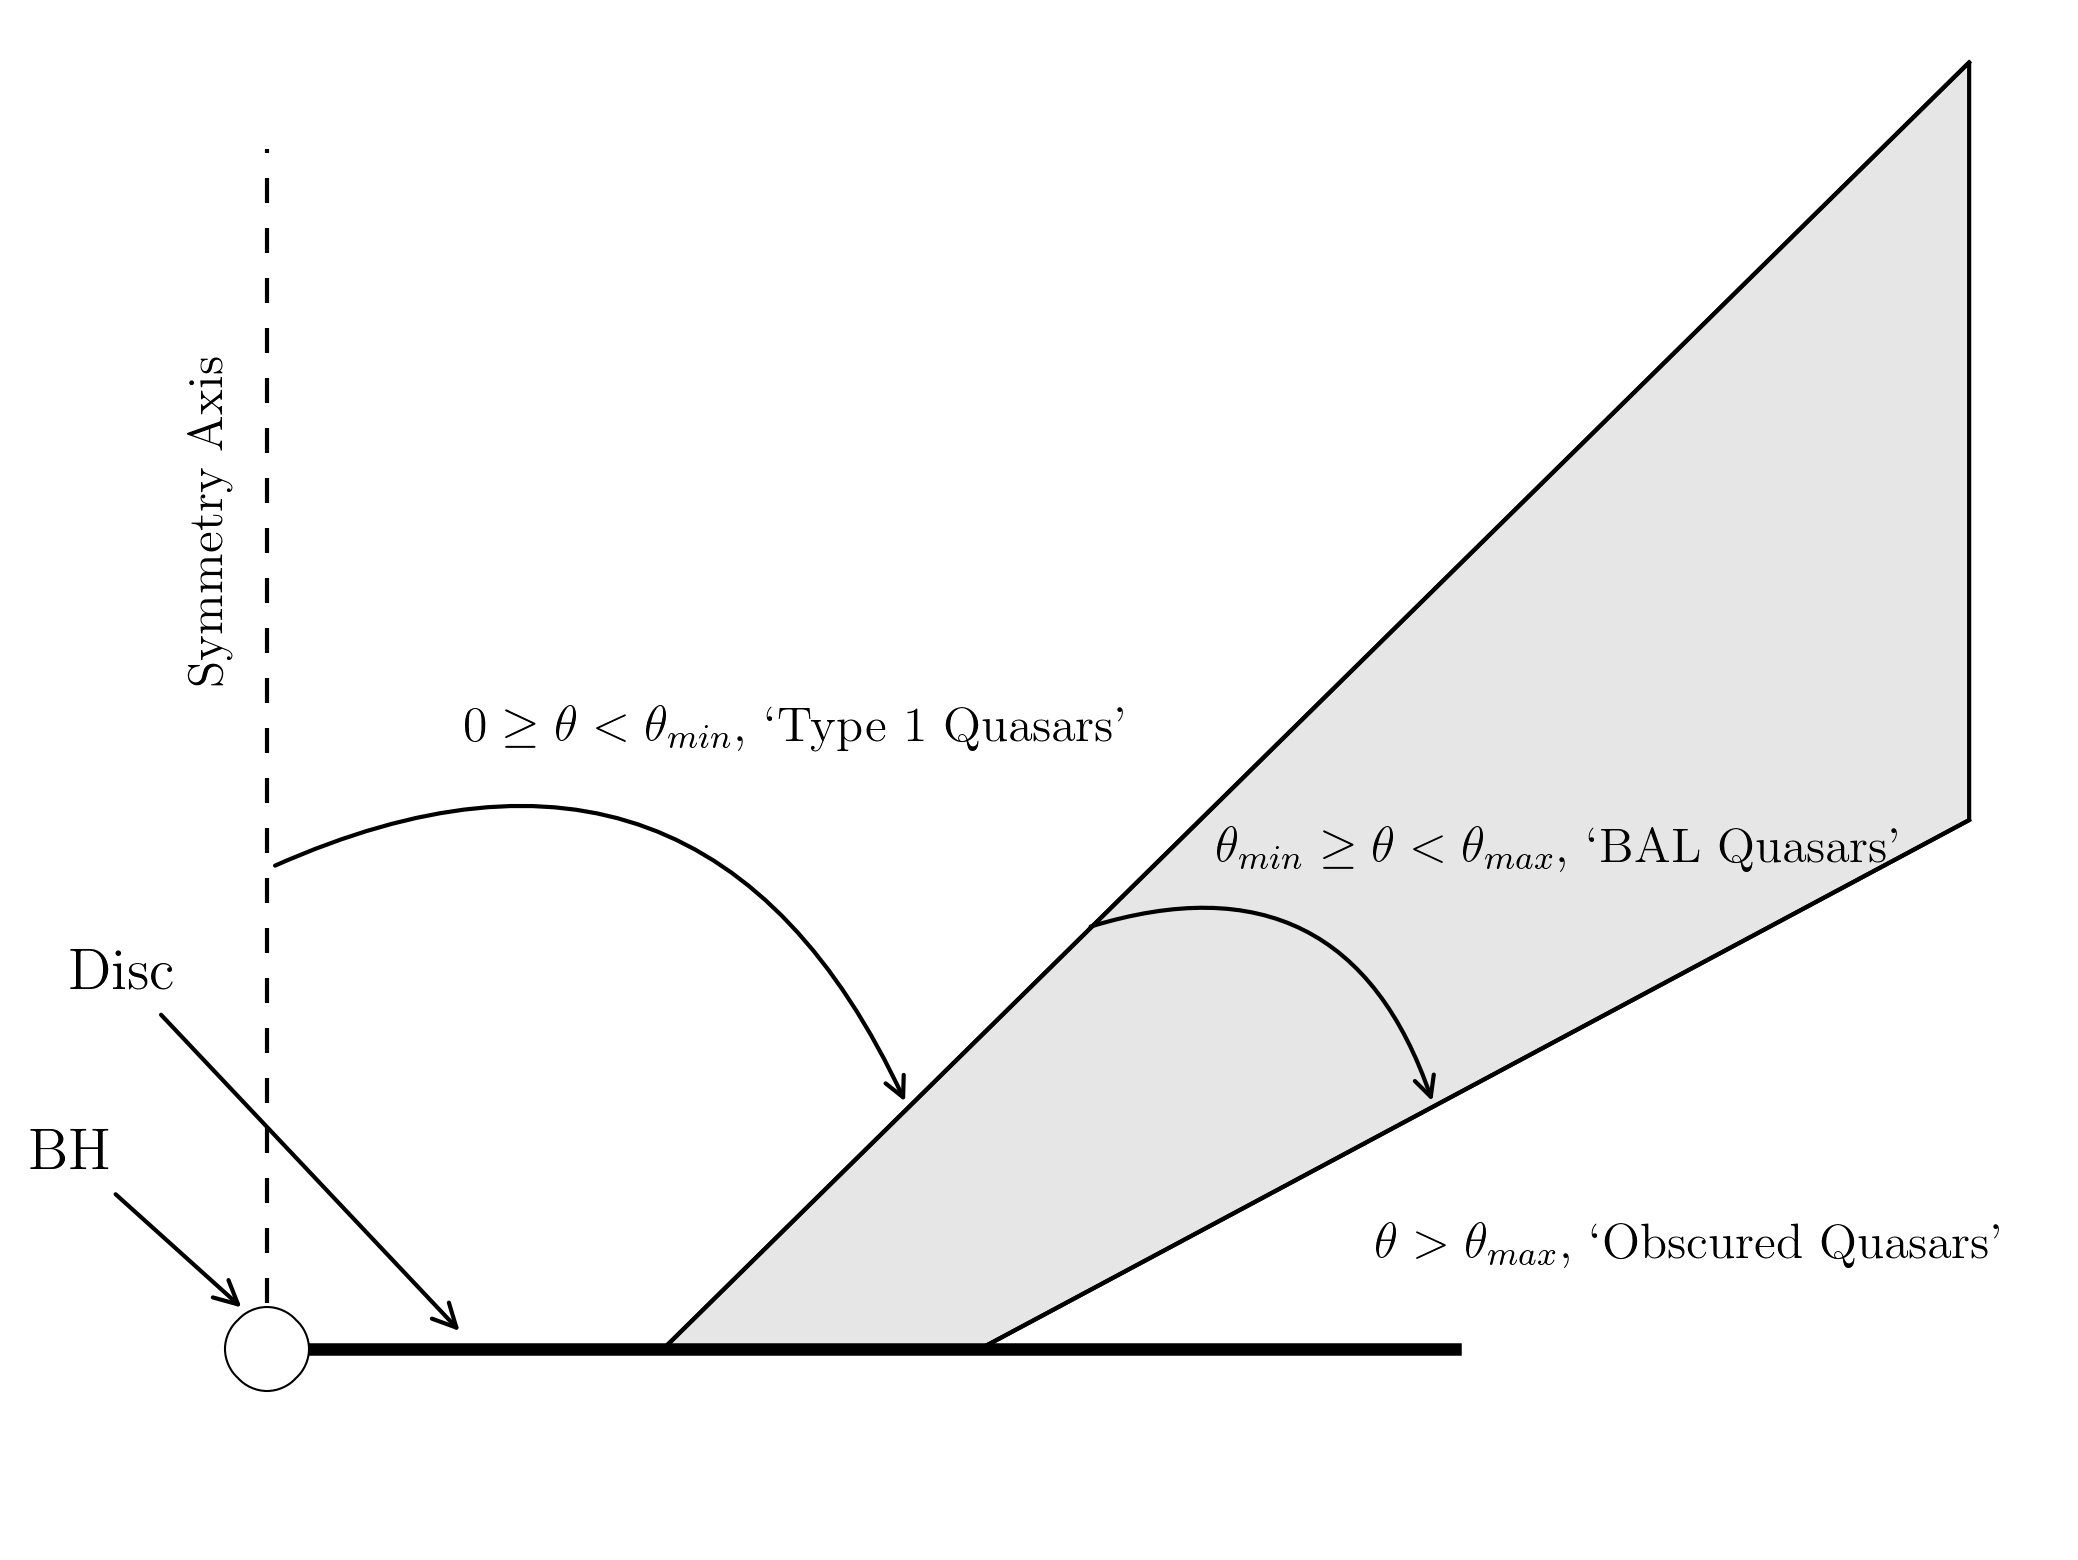
\includegraphics[width=0.8\textwidth]{figures/ewpaper/fig2_cartoon.png}
\caption
{
The geometry of the toy model used to carry out the Monte Carlo simulations
}
\label{fig:cartoon}
\end{figure}

% For LoBALs, \ewo\ measurements are available. This means the 
% non-BAL quasar \ewo\ distribution can actually be fitted in
% the LoBAL redshift range, and the expected LoBAL \ewo\ distribution
% predicted for a grid of $\theta_{min}$ and $\theta_{max}$. To do this,
% the procedure used to generate

In order to compare the observed distributions to those expected for LoBALs and
non-BALs I conduct a Monte Carlo simulation similar to
the process described in section~\ref{sec:fitting}, but with a few 
key differences. I once again assume $\epsilon(\theta) = \cos \theta$.
The geometry of the toy model used in this simulation is shown in
Fig.~\ref{fig:cartoon}.

First, A set of isotropic angles is generated.
If $\theta_{min}<\theta<\theta_{max}$ then the fake object 
is flagged as a mock BAL. If $\theta<\theta_{min}$ then the 
fake object is designated a non-BAL, and otherwise
the object is ignored. Once again, the object also has to 
survive a selection test based on a arbitrary flux selection limit.
I then fit the non-BAL distribution using the method described previously.
For each mock sample, a $\ew_*$ is drawn from the intrinsic gaussian,
and a mock EW is estimated such that $\ew = \ew_* / \epsilon(\theta)$.
This process is repeated to build up a mock sample of objects, and 
carried out for a series of pairs of $\theta_{min}$ and $\theta_{max}$.
This allows theoretical distributions for BAL and non-BAL quasars
for a series of different outflow geometries to be derived.

The diagnostics recorded from the simulation are the following four
quantities:
\begin{itemize}
	\item The $p$-value associated with a two-tailed Kolgomorov-Smirnov (K-S) 
	test statistic, $p_{KS}$, in which the mock BAL sample is compared
	to the real LoBAL sample.
	\item The BAL fraction, $f_{BAL}$, is calculated from the 
	number of objects in the mock sample with $\theta_{min}<\theta<\theta_{max}$.
	\item The $\chi^2/dof$ from the fit to the non-BAL quasar distribution.
	\item $\Delta \mu_{EW}$, the difference between the mean value of the mock BAL
	distribution and the mean value of the mock non-BAL distribution.
\end{itemize}
The simulation results are shown in figure~\ref{fig:contour}, in which the 
four diagnostics are plotted as a function of $\theta_{min}$ 
and $\theta_{max}$. 

As expected, equatorial viewing angles for LoBAL quasars 
are disfavoured, and furthermore, it is only possible to fit
the tail to the \ewo\ distribution if non-BAL quasars are allowed 
to be viewed from high inclinations. There is no region of parameter
space where a satisfactory fit is obtained to the quasar distribution
without simultaneously obtaining a large value of $\Delta \mu_{EW}$. The
K-S test allows us to reject the null hypothesis
The simulations favour a geometry in which BAL quasars are viewed
from very similar angles to non-BAL quasars.

The conclusions here are limited by the lack of knowledge about the 
intrinsic face-on distribution of \ewo, or equivalently,
the orientations of the quasars themselves. If either of these
quantities were known then the results of the
K-S test and $\chi^2$ minimization could be used
to place more robust constraints on BAL and non-BAL viewing angles 
and the associated covering factor of the outflow.
Furthermore, the distribution of \civ\ quasar EW cannot be fit by 
the same model as the \ewo\ distribution.
% Despite these difficulties, it is still relatively easy to 
% demonstrate that the EW distribution in BAL quasars is not well produced by a 
% model in which the accretion disc is foreshortened 
% and BAL quasars are viewed from high inclinations. I will show this byconducting
% a slightly simpler Monte Carlo experiment to ascertain which geometries 
% best reproduce the observed distributions.

% First, I find that the quasar EW distribution
% cannot be well-fitted unless quasars are viewed from a wide range of angles,
% right up to edge-on. This was already known from the analysis in 
% section~\ref{sec:fitting}. However, now we can see that this region of
% parameter space is the region most disfavoured when comparing the mock BAL
% dataset to the observed BAL dataset, and outflows occupying those
% opening angles would have significantly higher EWs than the non-BAL
% quasars.

% Although the quasar EW distribution can be fitted with the above 
% model, neither the true distribution of viewing angles 
% or the intrinsic `face-on' EW distribution of the emission line in 
% question is known. If an intrinsic, face-on distribution could be constructed
% then the Kologomorov-Smirnov test and $\chi^2$ minimization could be used
% to place constraints placed on BAL and non-BAL viewing angles.
% Furthermore, the distribution of \civ\ quasar EW cannot be fit by the same
% model as the \ewo\ distribution.
% Despite these difficulties, it is still relatively easy to 
% demonstrate that the EW distribution in BAL quasars is not well produced by a 
% model in which the accretion disc is foreshortened 
% and BAL quasars are viewed from high inclinations. I will show this byconducting
% a slightly simpler
% Monte Carlo experiment to ascertain which geometries best reproduce the observed
% distributions. Throughout these simulations, 

\begin{figure*} %fullpage
\centering
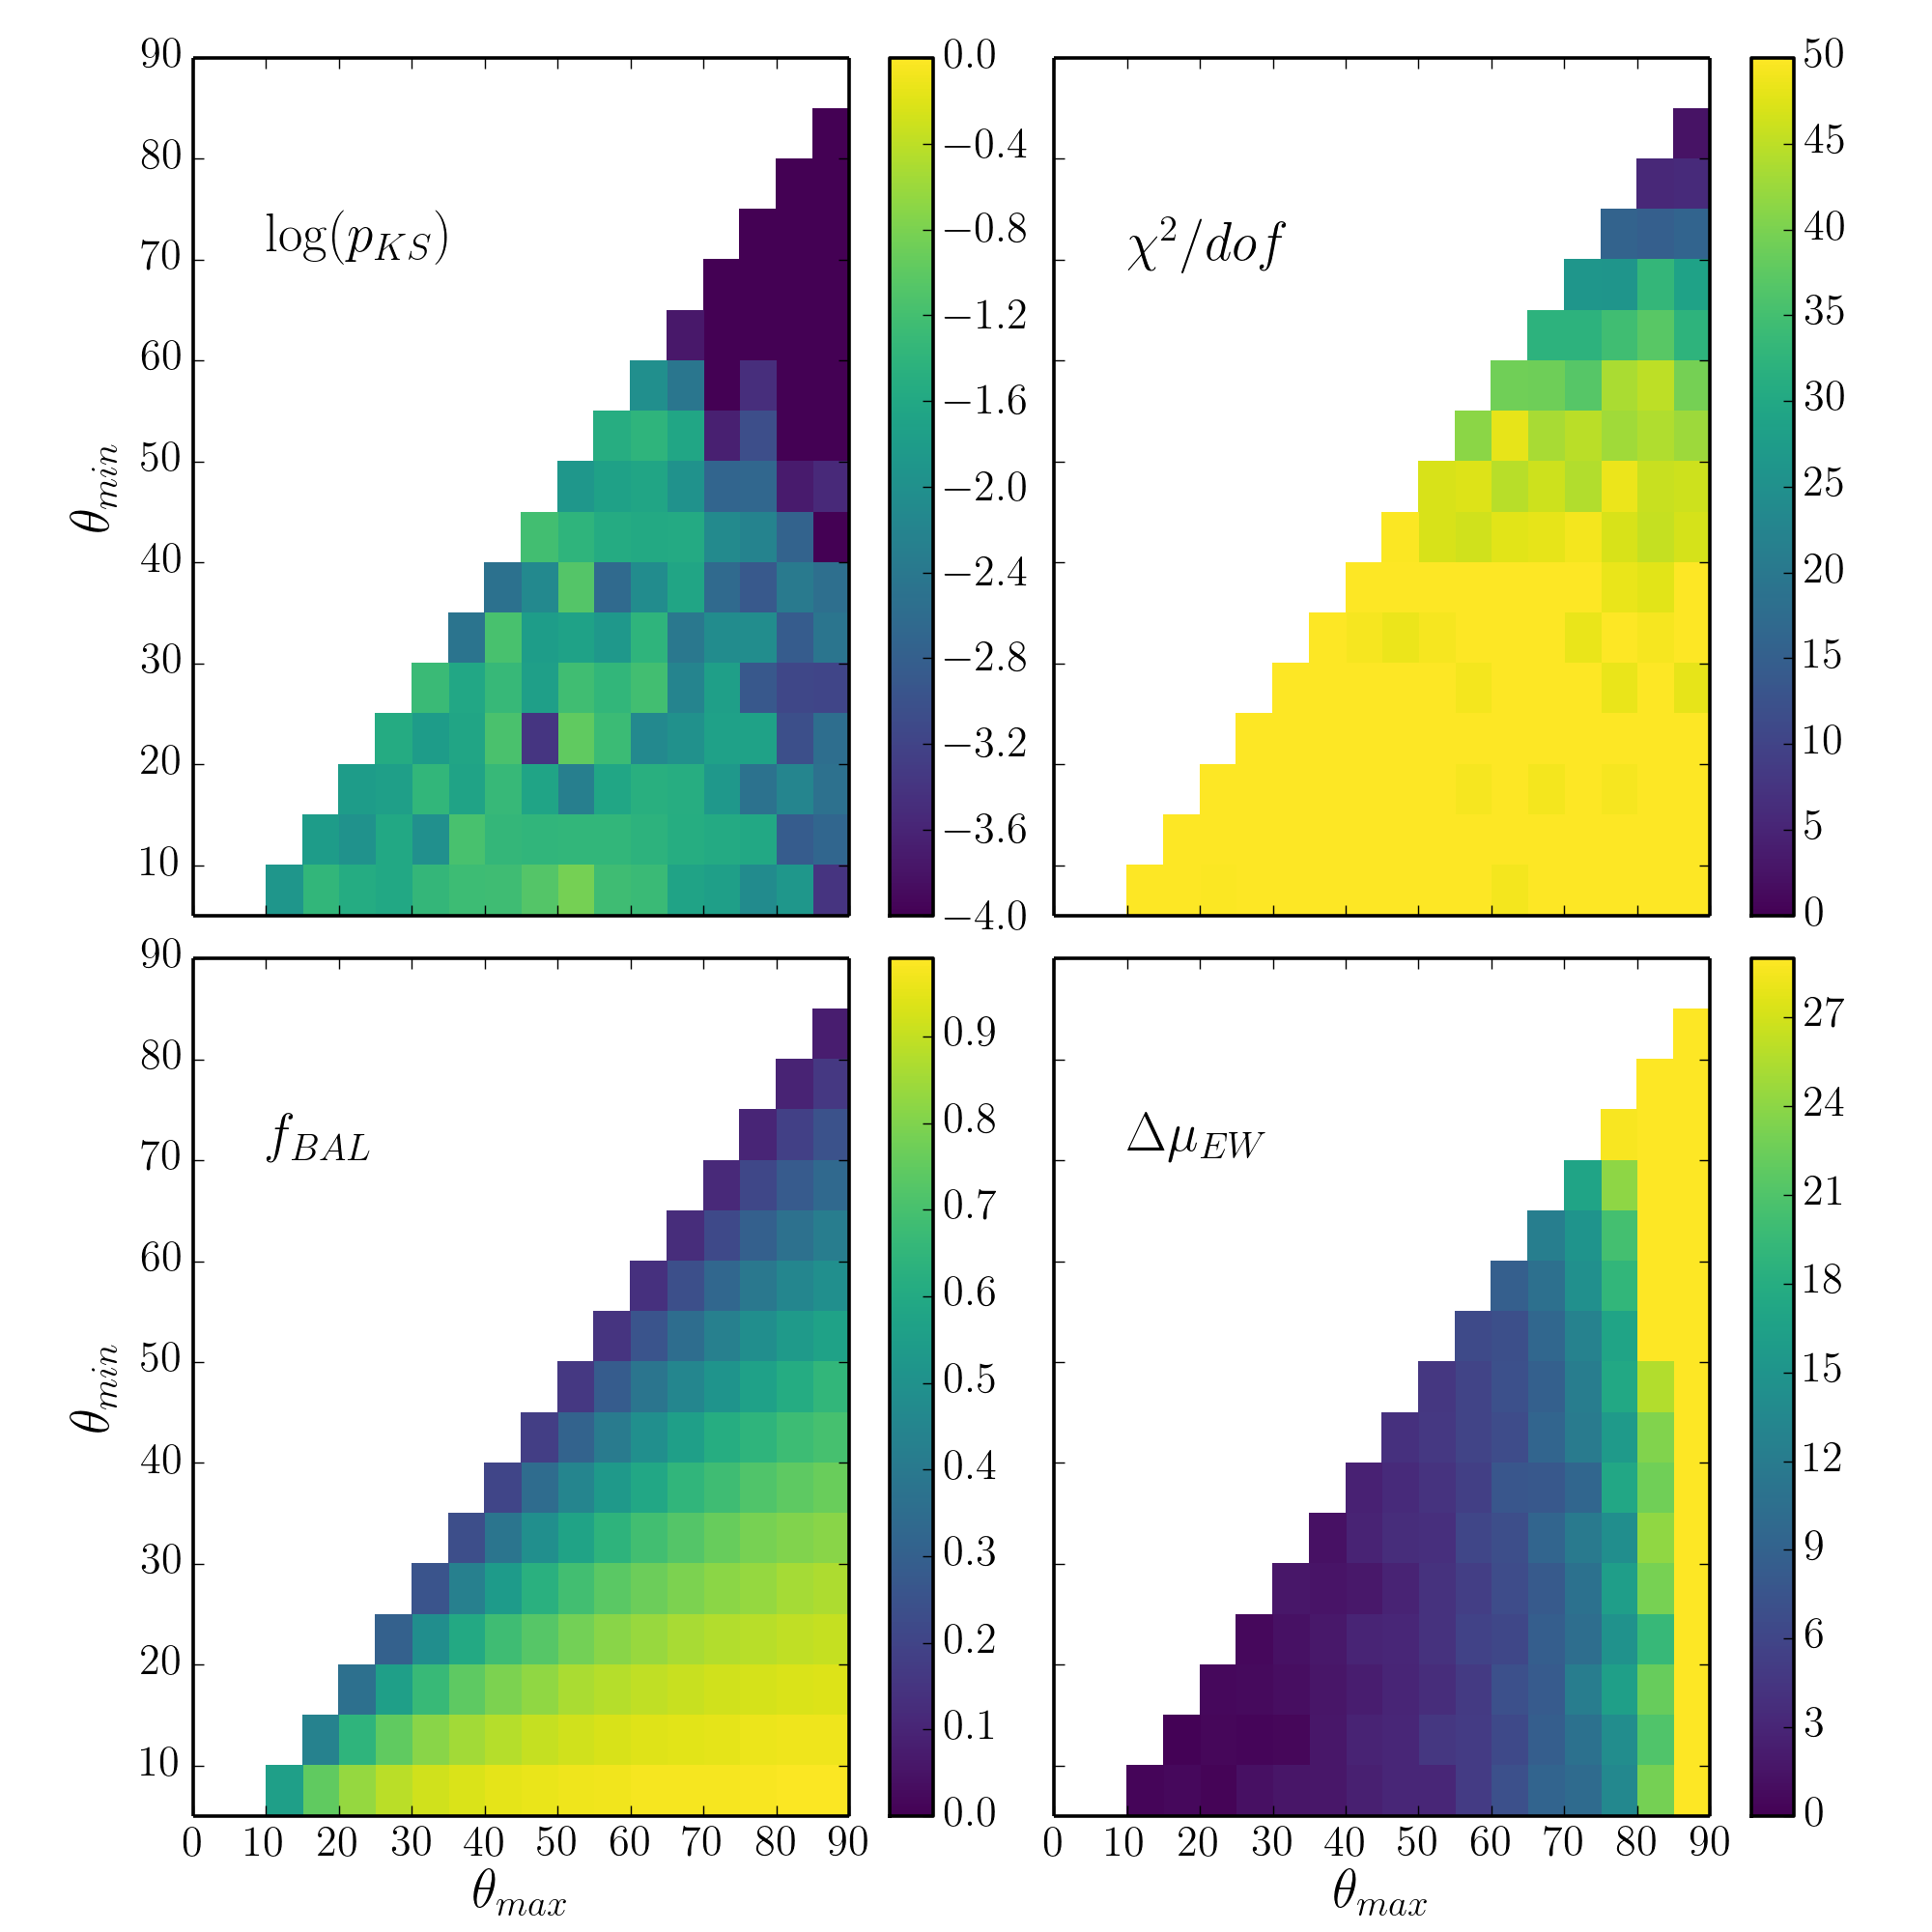
\includegraphics[width=1.0\textwidth]{figures/ewpaper/mesh4_ew_o3_max_sdss.png}
\caption
{
Heat map showing the results of the MC simulation described in 
section~\ref{sec:bal_v_nonbal}. The quantities shown are discussed 
further in the text, but correspond to (clockwise from top left):
the $p_{KS}$ value from a comparison between the mock BAL dataset
and the observed BAL dataset, the reduced $\chi^2$ from the fit to
the non-BAL EW distribution, the difference in mean EW between the 
mock BAL and mock non-BAL datasets, and the BAL fraction expected
for the geometry in question.
}
\label{fig:contour}
\end{figure*} %fullpage

An additional limitation is due to the SDSS wavelength coverage
and means that only LoBALs can be used when \ewo\ is present (sample A).
I would suggest that future observational programs might 
look to build up a large sample of \ewo\ measurements for HiBAL
quasars. In the mean time, I will turn to the UV broad emission
lines to examine if the above conclusions also hold
when examining the properties of the HiBAL quasars in sample B.

\subsection{Broad Emission Lines in HiBAL quasars: Theoretical EW Distributions for Sample B}
\label{sec:hibal_v_nonbal}

\begin{figure} %fullpage
\centering
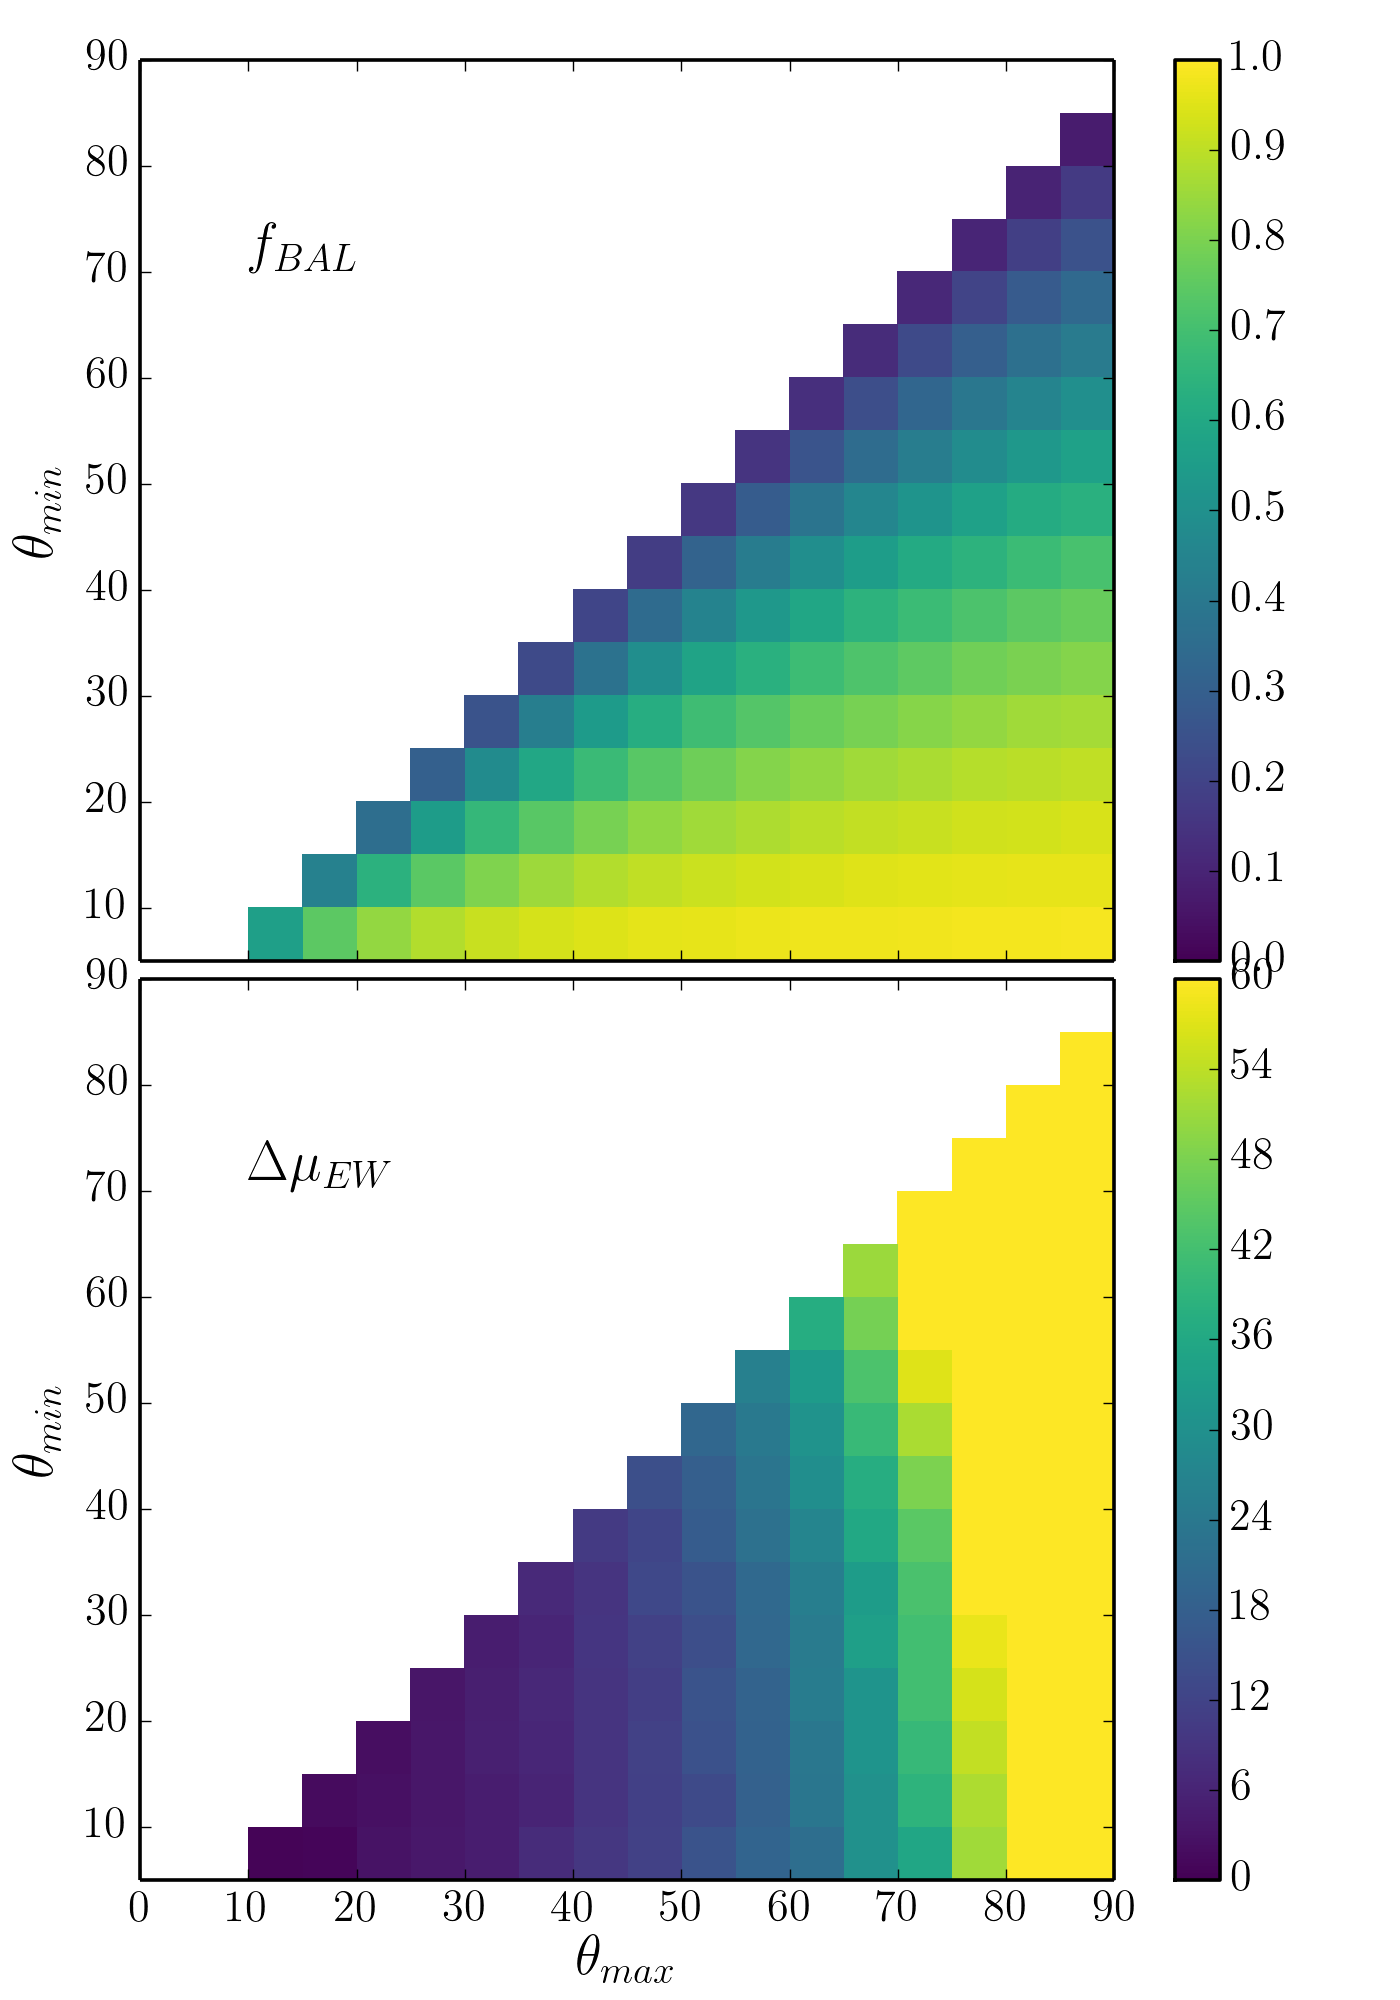
\includegraphics[width=1.0\textwidth]{figures/ewpaper/faceon_ew_c4_faceon_sdss.png}
\caption
{
Heat map showing the results of the MC simulation described in 
section~\ref{sec:hibal_v_nonbal}. The top panel shows the expected 
BAL fraction for the geometry in question, and the bottom
panel shows the difference in the mean value of the mock BALQSO distribution,
this term compared to the intrinsic non-BAL quasar distribution.
}
\label{fig:c4_faceon}
\end{figure} %fullpage

Unfortunately, it is not possible to produce a good fit to 
the non-BAL quasar \civline\ EW distribution using the above method 
(the best fit has $\chi^2/dof\approx8$).
This is due to the fundamentally different shape of the \civ\ EW distribution 
compared to \oiii. This difference in shape could be due to line opacity effects 
(see section~\ref{sec:line_aniso}) or obscuration of the BLR, which is significantly
more compact than the NLR (see section~\ref{sec:obscure}).
Thus, to explore which geometries are favoured by the \civ\ distribution,
I conduct a simpler test, in which I make the assumption that the intrinsic
distribution is roughly equivalent to the non-BAL quasar EW distribution.
I repeat the procedure from the previous section, but instead draw $\ew_*$
from the non-BAL quasar distribution. As I result, I only record $\Delta \mu_{EW}$
and $f_{BAL}$ as diagnostics. 

The results are shown in Fig.~\ref{fig:c4_faceon}. 
Similar trends are observed to those in LoBALs; geometries
in which BAL outflows emerge at extreme inclinations should produce
dramatically higher mean values for the EW, but this not seen in 
the data. Although this analysis makes more assumptions than for the \ewo\
fitting, it still implies that BALQSOs are not viewed from significantly 
higher inclinations than non-BAL quasars.


\section{Discussion}
\label{sec:discuss_ew}
I have demonstrated that the EW distributions of the 
\oiiifull\ emission line in LoBAL and non-BAL
quasars is not consistent with a 
model in which LoBAL quasars are viewed from equatorial angles 
and the continuum emission originates from
a foreshortened accretion disc. The EW distributions of 
\civline\ suggest that a similar conclusion applies to HiBAL quasars.
This result would be strengthened were 
I to include limb darkening. I will now explore how the above results compare to other
observations of quasars that might probe system orientation, as 
well as the potential impact of obscuration and line anisotropy
on the results.

\subsection{Eigenvector 1}

% \begin{table}
% \centering
% \begin{tabular}{p{2cm}p{2cm}p{2cm}p{2cm}}
% \hline Par. A & Par. B & $r_{corr,AB}$ (non-BALs) & $r_{corr,AB}$ (BALs) \\ 
% \hline \hline 
% $\log$[\ewo] & \fwh\ & 0.14 & 0.18 \\
% $\log$[\ewo] & $R_{{\rm Fe \textsc{ii}}}$ & $-0.51$ & $-0.67$ \\
% \fwh\ & $R_{{\rm Fe \textsc{ii}}}$ & $-0.26$ & $-0.42$ \\
% \end{tabular}
% \centering
% \caption
% [Eigenvector 1 correlation coefficients]
% {
% Eigenvector 1 correlation coefficients
% }
% \label{ev1_corr}
% \end{table}

Eigenvector 1 (EV1) is a fundamental parameter space for AGN and quasars
\citep{borosongreen,sulentic2000ev1,marziani2001,shenho2014}. 
It relates the FWHM of \hb, the relative iron strength, 
$R_{{\rm Fe \textsc{ii}}}$, and
\ewo. Both \ewo\ and \fwh\ have been used as orientation
indicators, and so comparing the LoBALQSO EV1 distribution to the non-BAL 
quasar EV1 distribution is particularly interesting. Once again,
HiBALs cannot be placed on this space due to the lack of rest-frame 
optical coverage.

Fig.~\ref{fig:bal_ev1} shows the quasar distribution from sample A 
in EV1 parameter space, with BAL quasars from samples A and B overplotted.
\cite[][hereafter SH14]{shenho2014} propose 
that the main inclination driver in the parameter space
is \fwh, and that high inclination sources should thus cluster around
a diagonal line from the lower right to upper left quadrants. In constrast,
R11's analysis predicts that high inclination sources should cluster
around high EW OIII widths. As \ewo\ and \fwh\ are very weakly correlated
(Spearman's rank coefficient of 0.14), this means they should lie to
the left of the parameter space. Inspection of the figure clearly 
shows that BAL quasars are not only found in one region of the 
EV1 parameter space. 

In order to assess this more quantitavely, I have shown contours of 
quasar counts overlaid on the scatter plot. The contours correspond
to the number of objects in each bin, where the bins are of size
$\Delta R_{{\rm Fe \textsc{ii}}} = 0.2$ and $\Delta$\fwh$=500$km~s$^{-1}$.
The percentage of quasars falling within the inner contour is 45\%, 
whereas only 18\% of LoBAL quasars fall in the space. Conversely, 24\% 
of BAL quasars fall outside the outermost contour compared to 10\% of 
non-BAL quasars. It would therefore appear that BAL 
quasars are preferentially clustered towards the high-mass and 
high-inclination end of EV1 space (under the interpretation of SH14).
This is further illustrated by Fig.~\ref{fig:bal_ev1_bins},
which shows the LoBAL fraction in the same bins, compared to the 
mean LoBAL fraction. This is again suggestive of an overdensity 
towards the upper right of the parameter space.
It is also clear that a unification picture in which BAL 
quasars are viewed exclusively from high inclinations is unlikely,
under both the R11 and SH14 interpretations. 

Larger datasets, preferably including HiBAL quasars with EV1 measurements, 
are needed in order to properly constrain the EV1 behaviour of BAL quasars.
However, overall, the behaviour of EV1 in LoBALQSOs slightly 
strengthens the conclusion that BAL quasars are not always viewed from 
extreme inclinations.

\begin{figure}
\centering
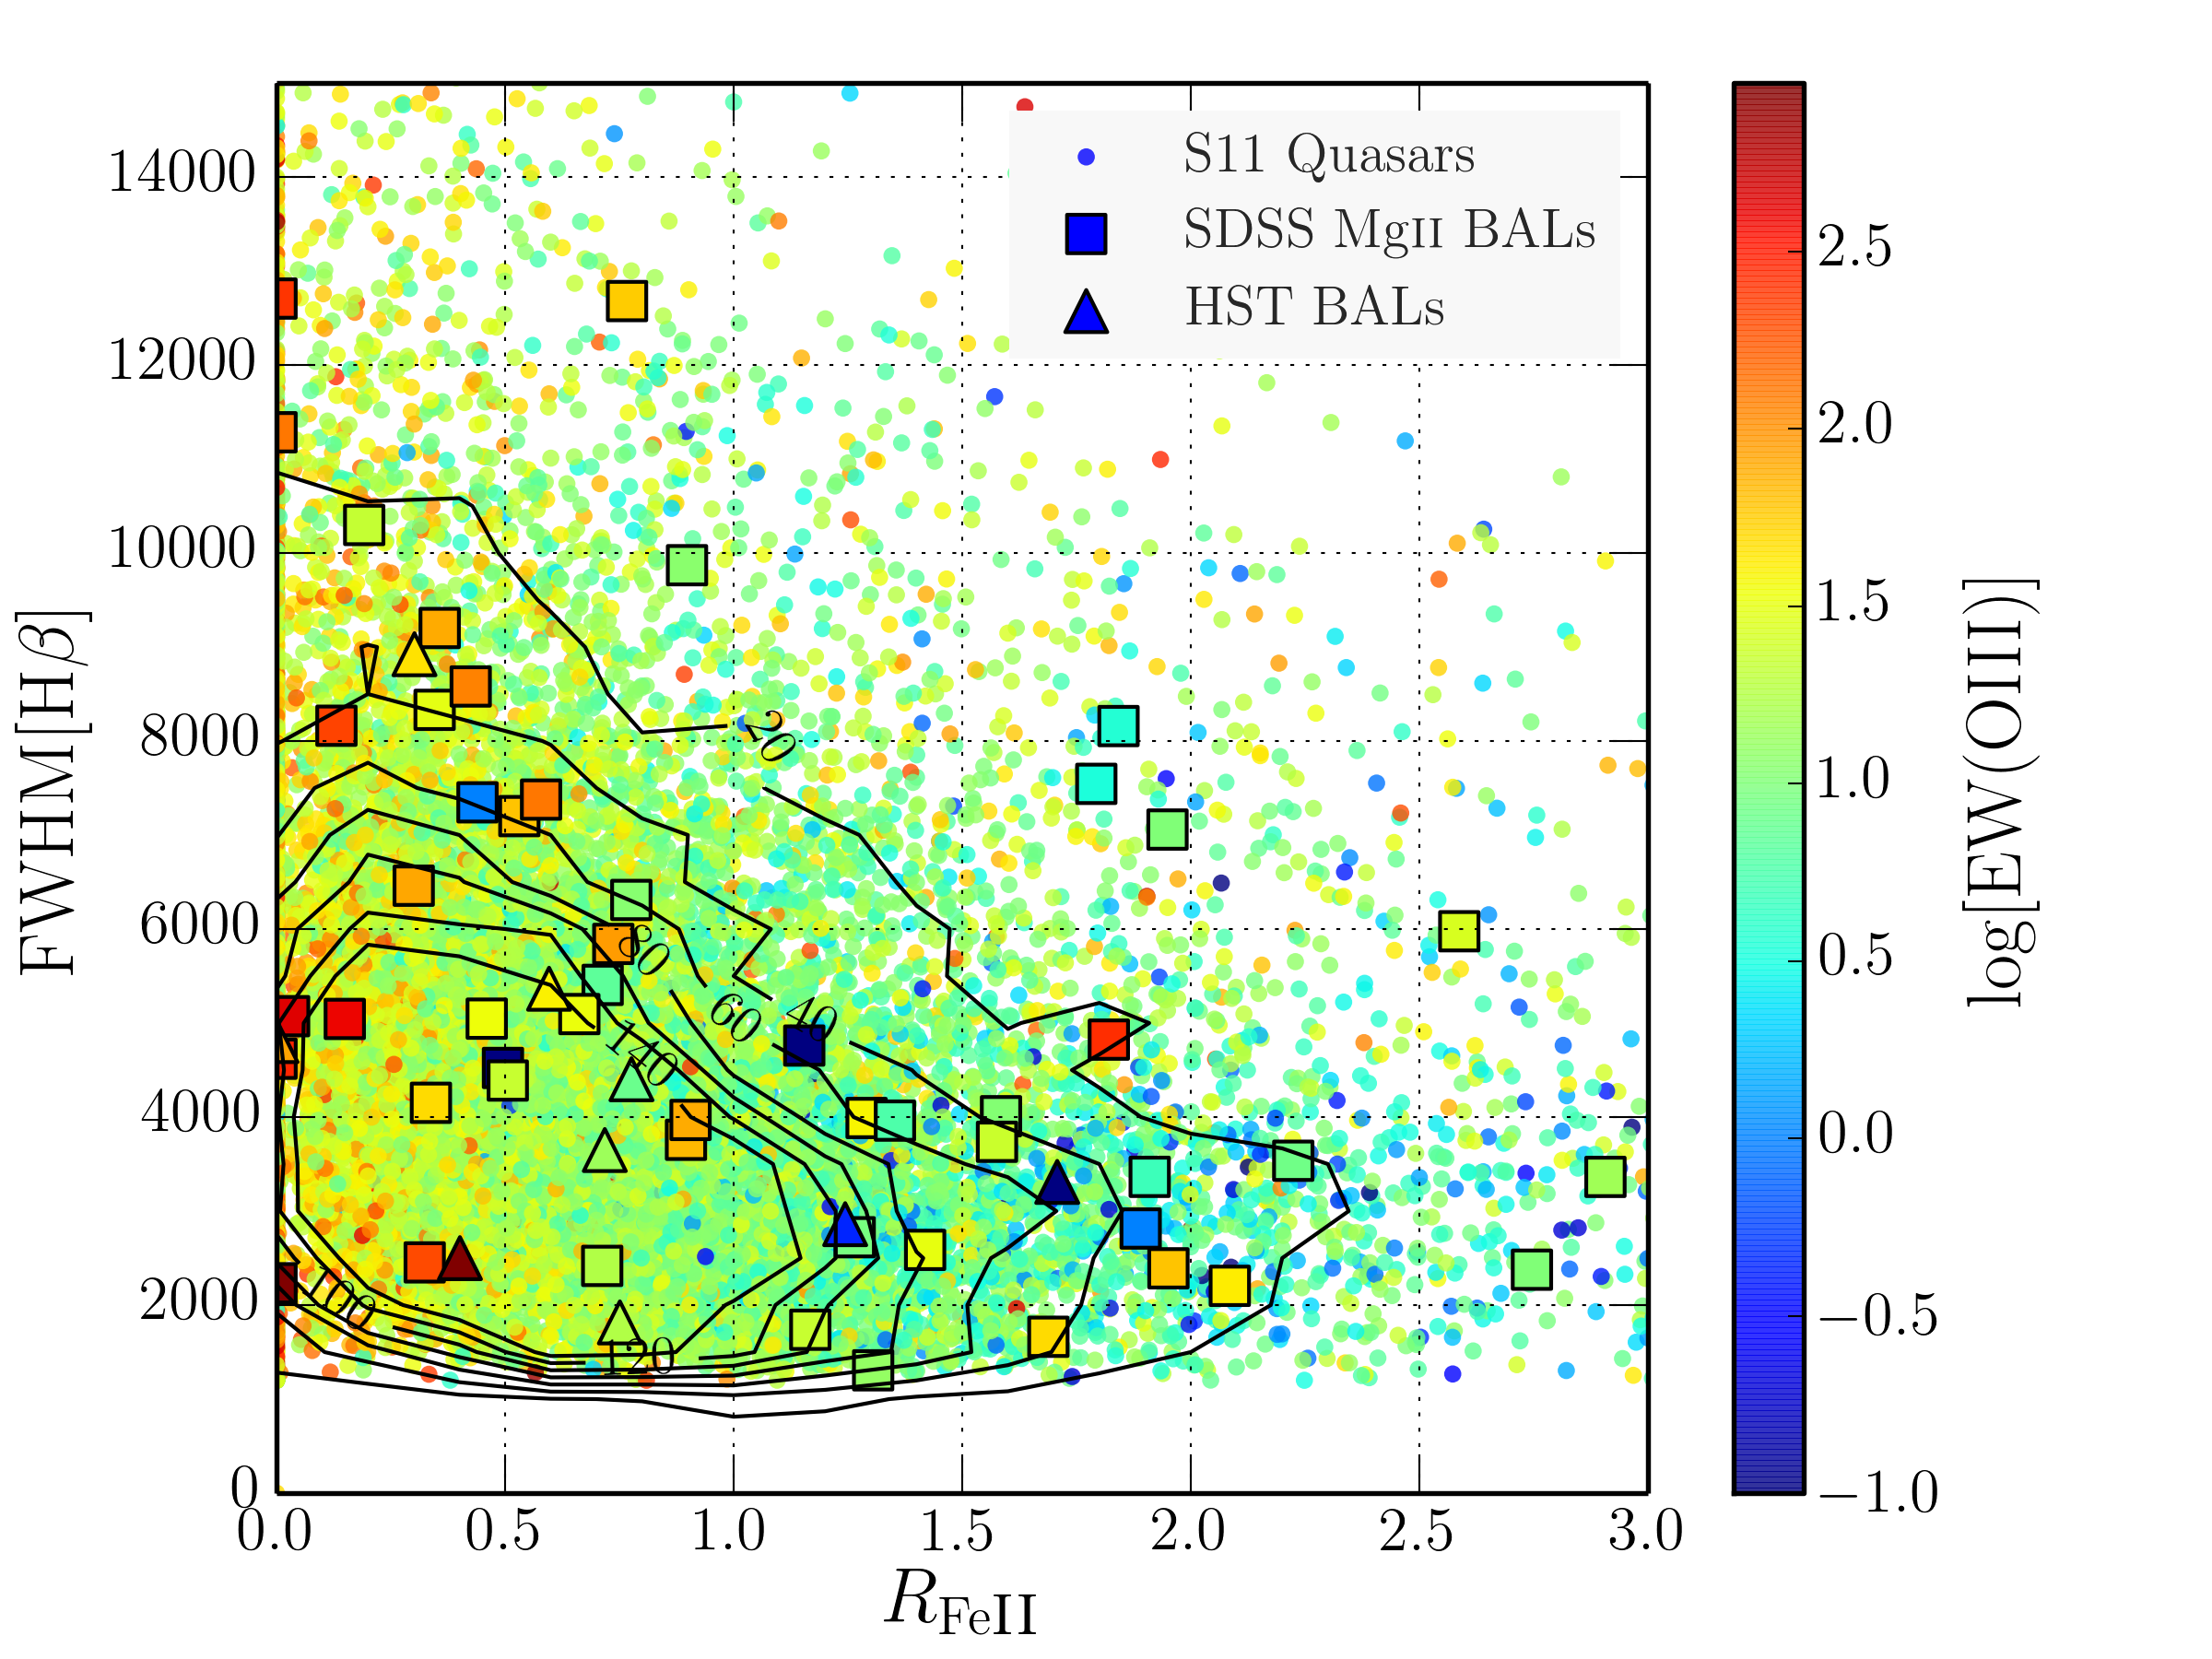
\includegraphics[width=0.8\textwidth]{figures/ewpaper/ev1.png}
\caption
[Eigenvector 1 for BAL and non-BAL quasars.]
{
Eigenvector 1 for BAL and non-BAL quasars. 
FWHM of the \hb\ line plotted against the relative
iron strength, $R_{{\rm Fe \textsc{ii}}}$. The colour coding
corresponds to the EW of OIII. The dots mark all quasars from
sample A, while the squares mark those with \mgii\ BALs.
The triangles show the HST BAL quasars from sample B.
}
\label{fig:bal_ev1}
\end{figure}

\begin{figure}
\centering
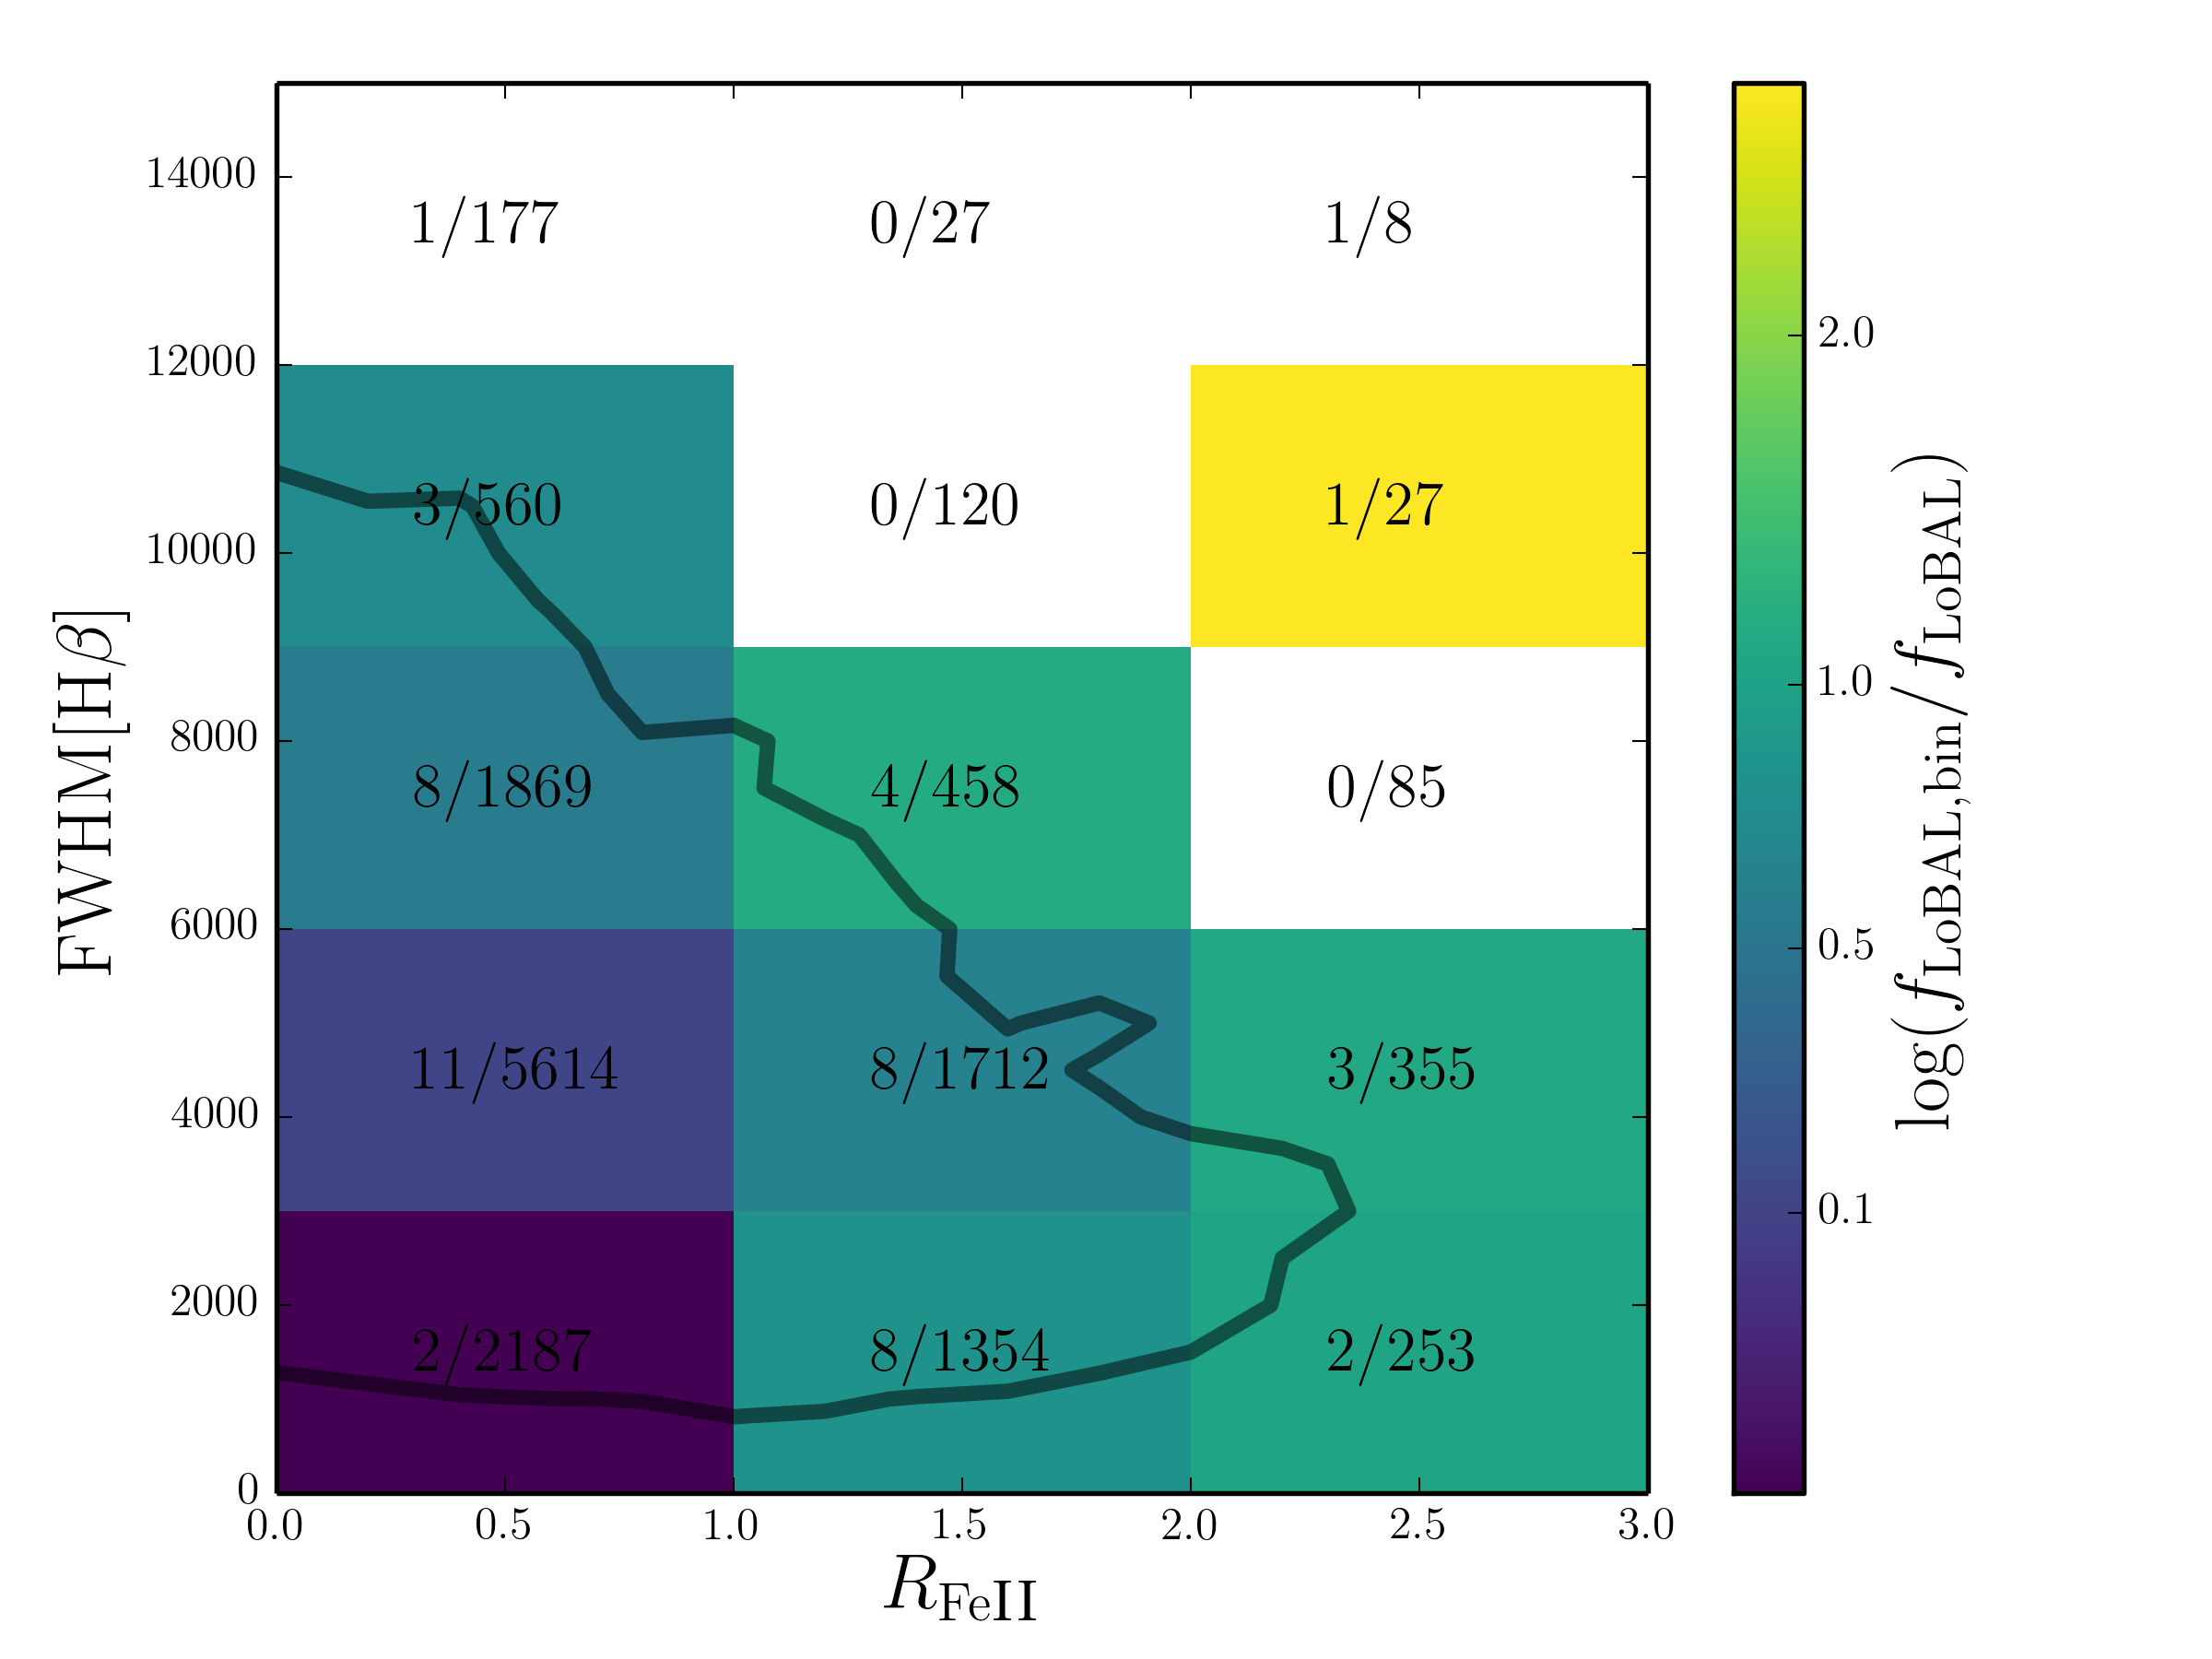
\includegraphics[width=0.8\textwidth]{figures/ewpaper/ev1_bins.png}
\caption
[LoBAL fraction compared to mean LoBAL fraction in Eigenvector 1 space.]
{
LoBAL fraction compared to mean LoBAL fraction in Eigenvector 1 space.
The contour shows the outermost contour from Fig.~\ref{fig:bal_ev1} for
reference.
}
\label{fig:bal_ev1_bins}
\end{figure}

% \begin{figure}
% \centering
% 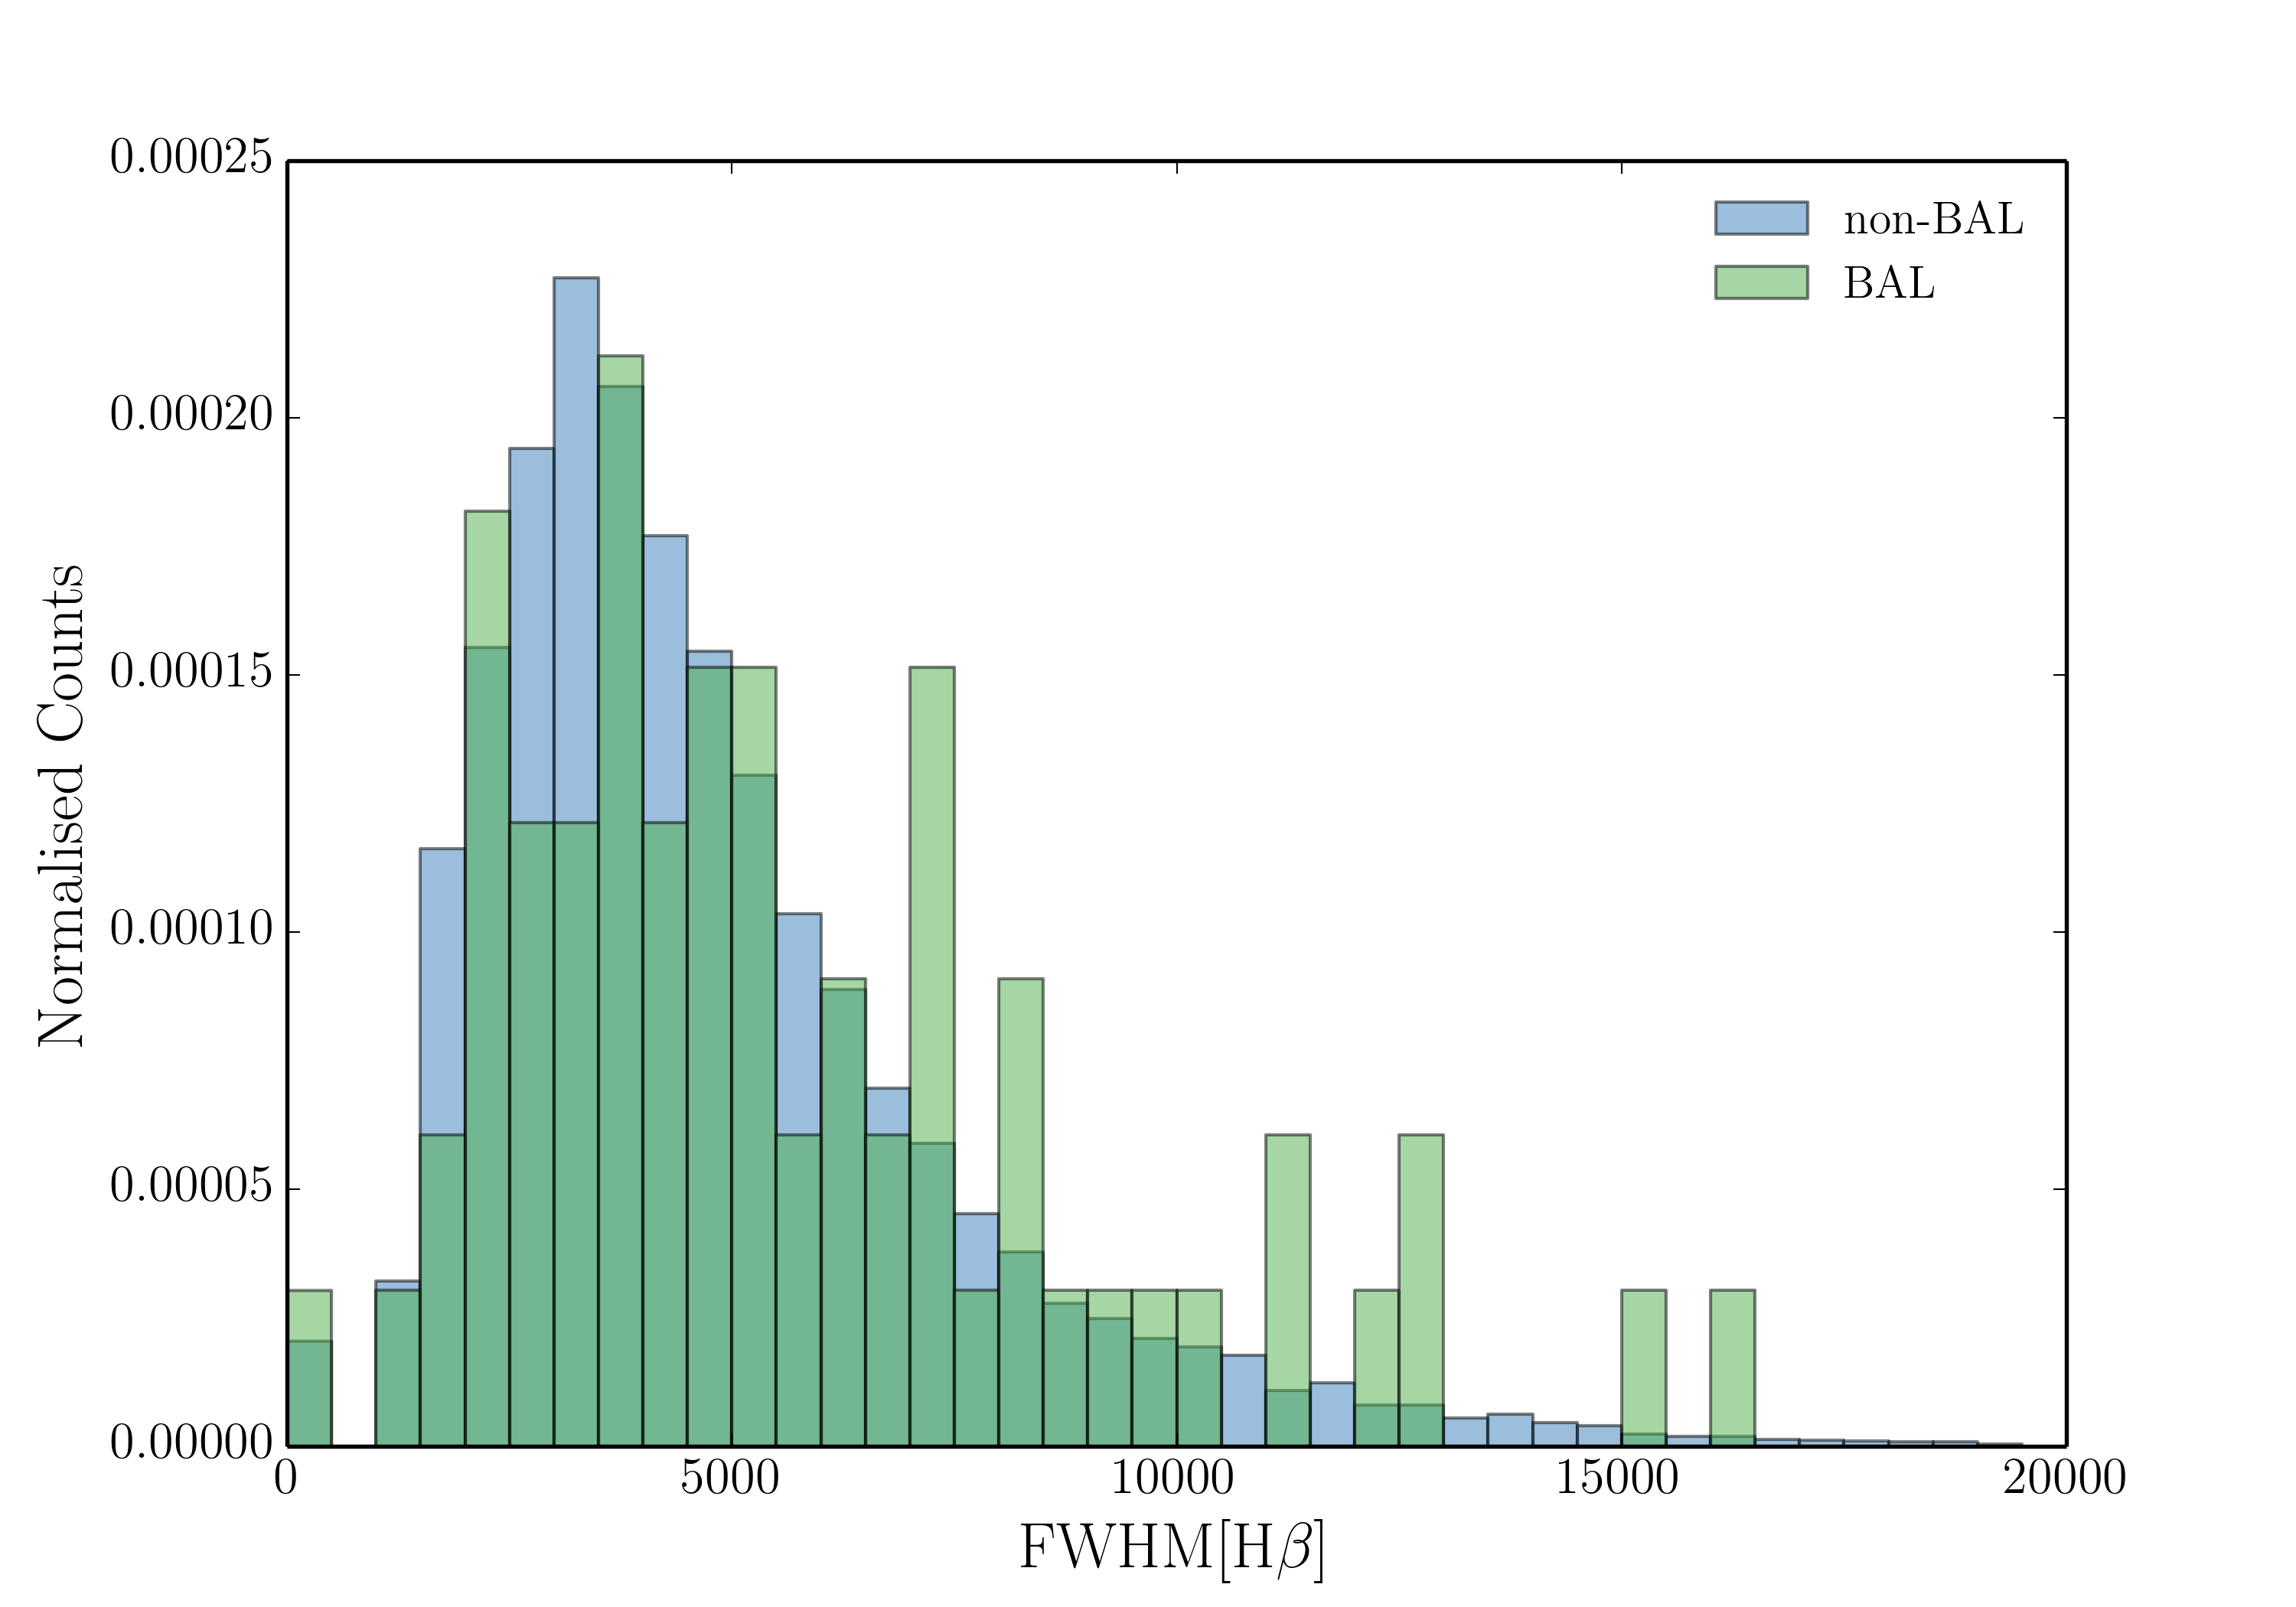
\includegraphics[width=1.0\textwidth]{figures/ewpaper/fwhm_hist.png}
% \caption
% [Distribution of \fwh\ in BAL and non-BAL quasars.]
% {
% Distribution of \fwh\ in BAL and non-BAL quasars.
% }
% \label{fig:fwhm_hb}
% \end{figure}
% \subsection{Radio Observations}
% Fig.~? shows the equivalent width distributions in radio-loud quasars, 
% split into core or lobe dominated. This designation is commonly used
% as an orientation indicator \citep{orr1982,wills1995}. 
% Although th
% In this case, we can see that 
% A full investigation of this is beyond the scope 
% {\color{blue}
% Alternative geometries and polarisation. Are there any problems with
% a more moderate viewing angle for BALs? Do we want to show a cartoon?
% Discuss modelling work. Also discuss compton-thick fraction at high mass end.
% What about PHYSICS. Can we derive lower limits on outflow angles from
% e.g. conservation of angular momentum??
% }


\subsection{Polarisation}

Spectropolarimetry of BAL quasars offer some of
the best insights into the geometries of BAL outflows, and 
tends to show a few key properties. The first is enhanced 
polarisation in the BAL troughs themselves \citep{schmidt1999}. 
This is readily explained by a scattering region unobscured by the
BAL trough, with the higher polarisation percentage simply due to the
decreased direct flux. This may also explain the non-black saturation in
BAL troughts (see section~\ref{sec:balqso_angles}).

The second property 
is a continuum polarisation percentage of around $2.4$ times greater, 
on average, than the non-BAL population \citep{schmidt1999}.
The continuum polarisation percentages of a sample of BAL quasars from 
\cite{schmidt1999} are compared to the Type I and Type II AGN 
populations from \cite{marin2014} in Fig.~\ref{fig:bal_polarisation}.
As we can see, BAL polarisation percentages lie between those of type 1
and type 2 AGN. If type 1 and type 2 objects are viewed from low and high 
inclinations respectively, as expected from unified models and measured by
\cite{marin2014,marin2016}, this is suggestive of an intermediate inclination
for BALQSOs. This enhanced polarisation is also well reproduced by intermediate
inclination flows in simple radiative transfer models \citep{marin2013}.

\begin{figure}
\centering
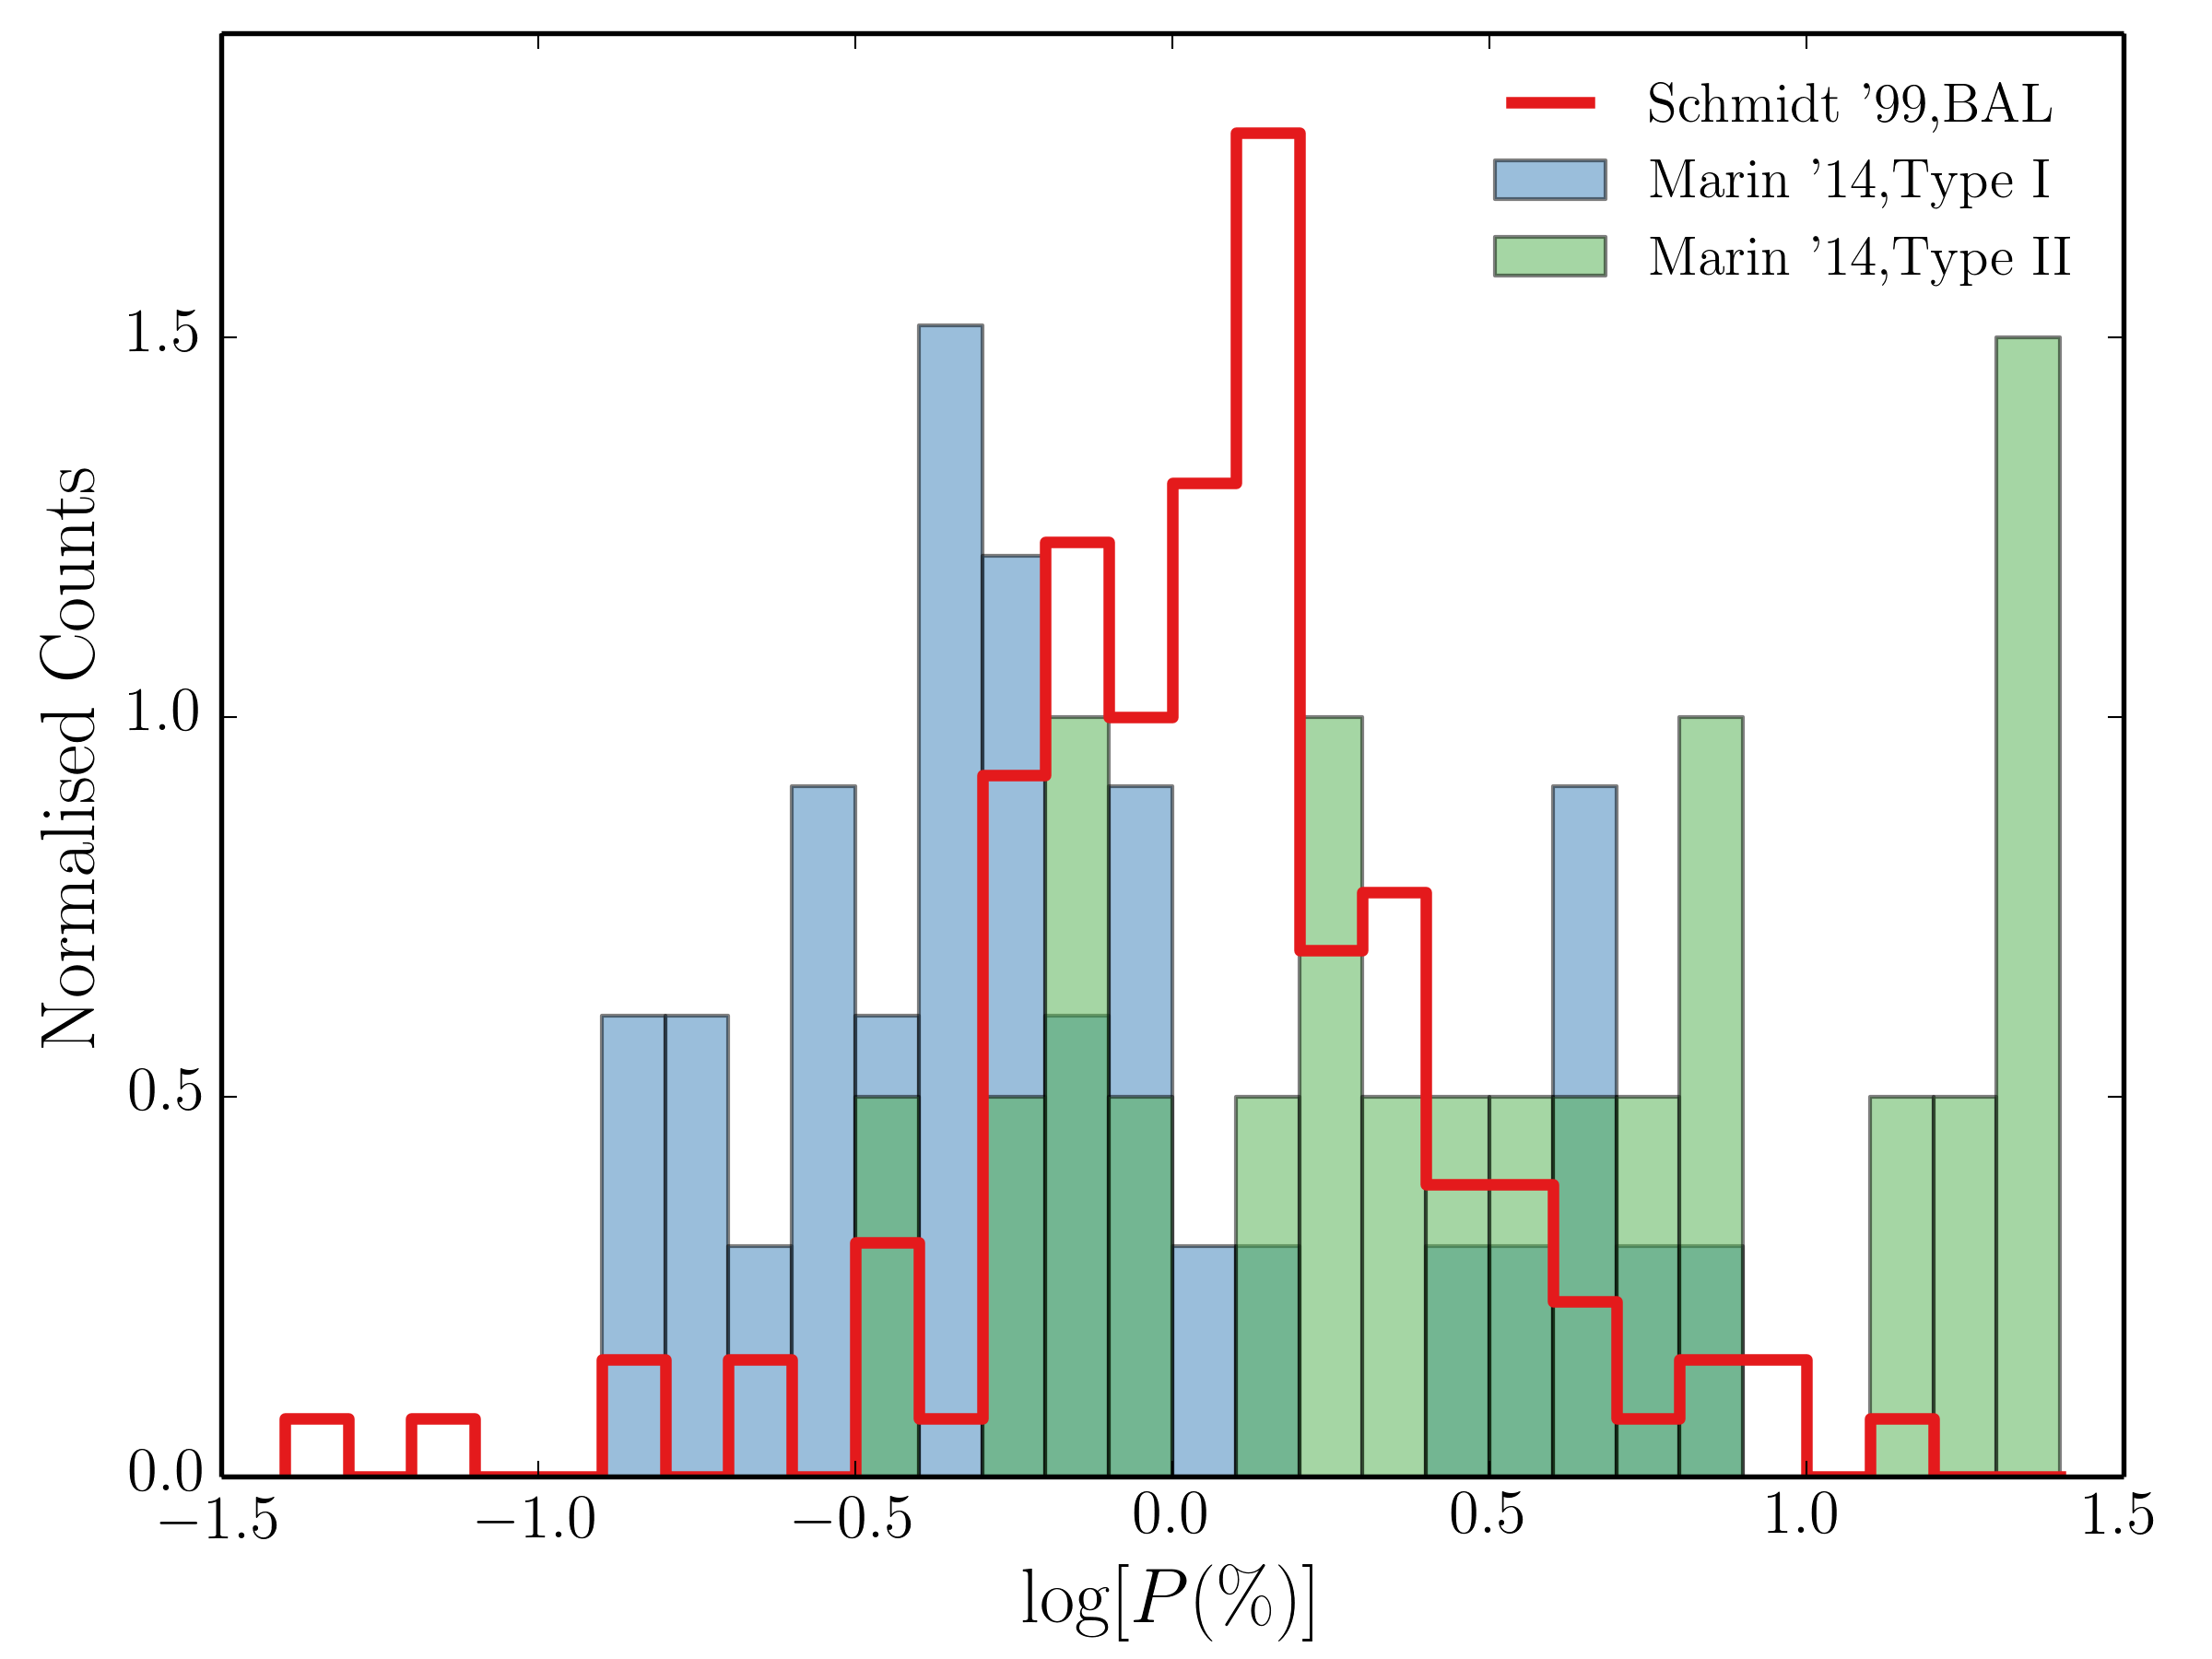
\includegraphics[width=0.9\textwidth]{figures/ewpaper/hist_p2.png}
\caption
{
Histograms of polarisation percentages 
for BAL quasars from Schmidt et al. (1999) together with the 
Marin et al. (2014) AGN sample. 
}
\label{fig:bal_polarisation}
\end{figure}

The third property is a polarisation angle of $\gtrsim60^\circ$ with respect
to the radio jet axis in RL BALQSOs \citep[][and references therein]{brotherton2006}.
This suggests a higher inclination (compared to non-BAL quasars)
viewing angle for BALQSOs under the interpretation of a geometric model. Indeed,
early polarisation studies explained the observations with a polar scattering region,
viewed at an equatorial angle 
\citep[e.g.][]{goodrich1995, cohen1995,lamy2004}. Regardless of
the true geometry, the reason for the difference must be understood.
I would suggest that polarisation predictions are made from wind
models such as the one I presented in chapter 5, using a similar
approach to \cite{marin2013}, but considering BALs in more detail. 
Overall, however, polarisation measurements imply that BAL quasars are viewed
from higher inclinations if the unified models are correct, and are 
in slight tension with the idea that BAL quasars are viewed from the same range
of angles as non-BAL quasars.

\subsection{The Effect of Obscuration}
\label{sec:obscure}

\cite[][hereafter C11]{caccianiga2011} showed that the distribution of \ewo\
can also be well fitted by an obscuration model. They modelled the 
\ewo\ distribution using an absorption model based on column densities
obtained from the {\sl XMM Newton} Bright Serendipitous Source (XBS)
sample. They use a sample size of 169 objects, and find that AGN with 
column densities of $N_H\gtrsim10^{22}$~cm$^{-2}$ can explain the high
EW powerlaw tail. 

The column density measurements BAL quasars suggest that obscuration 
cannot explain the distribution of \ewo\ in quasars. 
As briefly discussed in chapter 5, BALs generally show
strong X-ray absorption with column densities of $N_H\gtrsim10^{23}$~cm$^{-2}$
\citep{green1996,mathur2000,green2001,grupemathur2003}. \cite{gallagher1999}
found all BAL quasars in a sample of 7 had $N_H>10^{22}$~cm$^{-2}$, placing
them firmly in the EW tail according to the C11 model. This is broadly
consistent with the mean value of $3.5\times10^{22}$~cm$^{-2}$ from
\cite{marabito2014}, and would imply that BALQSOs should have significantly
higher EWs if obscuration governs the \ewo\ distribution.
Of course, only LoBAL quasars had \ewo\ measurements 
in the sample used here -- this actually strengthens the conclusion as low ionization 
BALQSOs show even higher column densities approaching Compton-thick values 
\citep{morabito2011}.


\subsection{Line Anisotropy}
\label{sec:line_aniso}

Optically thin lines are isotropic -- the {\em local}
escape probabilities in each direction are equal due to the 
low optical depth. 
When lines are optically thick, the situation is more
complex, as local velocity gradients then determine the line 
anisotropy. Indeed, Keplerian velocity shear has been shown to modify the
shape of disc-formed emission lines \citep{hornemarsh1986}, and an additional
radial shear from a wind could caused double-peaked lines
to become single-peaked \citep{MC96,MC97,flohic2012}.

R11 suggested that the broad emission lines trace the disc
emission in terms of their anisotropy. 
If this was the case, then we would not expect a difference in the BAL and non-BAL
quasar EW distributions. However, an emission line would only be purely 
foreshortened if emitted from a {\em static} disc. For broad emission lines
this is not true by definition. If the lines came from a region subject to
Keplerian velocity shear then the surface brightness of an optically thick 
line is \citep{hornemarsh1986}
\begin{equation}
J_{thick} \approx \cos \theta~S_L~\Delta \nu~\sqrt{8 \ln \tau_0},
\end{equation}
where $S_L$ is the line source function and
$\tau_0$ is the line centre optical depth, given by
\begin{equation}
\tau_0 = \frac{{\cal W}}{\sqrt{2}\pi \Delta \nu \cos \theta}.
\end{equation}
The parameter ${{\cal W}}$ is given by
\begin{equation}
{{\cal W}} = \frac{\pi e^2}{m_e c}f N^\prime,
\end{equation}
where $f$ is the oscillator strength and $N^\prime$ is the number
density integrated along the vertical height of the disc. The linewidth
$\Delta \nu$ is enhanced from the thermal linewidth by the velocity shear, such
that
\begin{equation}
\Delta \nu = \Delta \nu_{th} \left[1 + 
\left(\frac{3}{4}\frac{v_{k}}{v_{th}}\frac{H}{R}\right)^2
\sin^2 \theta \tan^2 \theta \sin^2 2 \phi
\right]^{1/2}.
\end{equation}
Here, $\phi$ is the azimuthal angle in the disc, $\nu_{th}$ and $v_{th}$ are the 
thermal line width in frequency and velocity units respectively, 
$H$ is the scale height of the disc at radius $R$, and $v_k$ is the
Keplerian velocity.

The outcome of the \cite{hornemarsh1986} analysis is that optically thick lines 
formed in a Keplerian disc are strongly anisotropic, but they do not follow a simple 
$\cos \theta$ distribution. Instead, the angular emissivity function is
a strong function of the velocity shear in the disc, the atomic physics of
the line in question, the location of the line formation region 
and the vertical disc structure. It is hence possible
that the broad emission lines are strongly anisotropic, and the presence of radial
velocity shear from a wind would only complicate matters. 
I would therefore suggest that future efforts might include fully modelling 
the line emission as a function of inclination to feed into the above analysis.

Regardless of the precise angular distribution, 
line emission should not trace disc emission
exactly, as we already know large-scale velocity fields are dynamically important
in the BLR, purely from the line widths. In that case, one would expect systematic
differences in EW between high inclination and low inclination sources, and these are 
not seen in the \civline\ and \mgline\ EW distributions.

\section{Conclusions}
\label{sec:ew_conclusions}

I have explored the emission line properties of BAL and non-BAL quasars,
particularly focusing on the EW distributions in two redshift ranges of the SDSS
quasar catalog. My main conclusion is simply that the EW distributions of BAL and
non-BAL quasars are remarkably similar, and this is not what one would expect from
a unification model in which an equatorial BAL outflow rises from a foreshortened 
accretion disc. This geometry has been used extensively in 
geometric unification and BAL outflow models in the past 
\citep[e.g.][]{MCGV95,PSK2000,PK04,risalitielvis2010,borguet2010,
higginbottom2013, nomura2013,nomura2016}, and was even adopted earlier in this thesis.
I then established that an angular emissivity function of \ept$=\cos \theta$ 
is actually the conservative estimate from thin disc models, and used this
to conduct a series of simulations similar to those conducted by \cite{risaliti2011}.
As expected, these simulations confirmed the above finding.

Based on this analysis, it is possible to construct a few possible scenarios 
that favoured by the above results. These conclusions have the caveat that I 
have assumed that conclusions drawn about LoBAL quasars can be extended to BAL 
quasars in general.
\begin{itemize}
	\item {\sl Scenario 1:} The quasar continuum is much more isotropic than one would
	expect from a geometrically thin, optically thick accretion disc.
    I have demonstrated that general relativistic effects cannot account for this discrepancy in the 
    UV. Reprocessing by surrounding dense plasma with a large covering factor or limb brightening 
    in the disc may provide possible explanations which this analysis cannot yet confirm or refute.
    \smallskip
	\item {\sl Scenario 2:} Quasar discs are strongly anisotropic, as expected from a 
	geometrically thin, optically thick accretion disc. In this case, BAL outflows cannot 
	only emerge at extreme inclinations and should instead be seen at very similar angles
	to non-BAL quasars. Polarisation measurements need to be reconciled with this hypothesis.
	I recommend that future RT modelling efforts explore different outflow 
	geometries and that detailed polarisation modelling is undertaken to constrain the 
	outflow opening angles.
	\smallskip
	\item  {\sl Scenario 3:} The geometric unification model does not explain the incidence of 
	BALs in quasars, or requires an additional component which is {\em time-dependent}, 
	such as an evolutionary or accretion state origin for BAL outflows. In this scenario, 
	BAL quasars would be seen from very similar angles to non-BAL quasars. If this is the case,
	the covering factors and opening angles of the outflows still need to be constrained so
	that feedback efficiencies can be accurately estimated.
\end{itemize}
I have confirmed that obscuration cannot explain the EW distributions of all quasars
due to the high column density observed in BAL (and particularly LoBAL) quasars. It is
possible that line opacity could explain the observed similarities between the broad emission
line distributions, but this cannot explain the similarities in the LoBAL and non-BAL
quasar \ewo\ distributions, as \oiii\ is a forbidden, optically thin transition.

Regardless of the conclusions about BAL quasars and their outflow geometries,
this analysis allows conclusions to be drawn about the {\em overall} 
quasar population. In scenario 1, the \ewo\ distribution of quasars cannot
be driven by inclination as suggested by \citep{risaliti2011}. This would
imply that \ewo\ is a poor orientation indicator. The lack of correlation 
between \ewo\ and \fwh\ also suggests that it is not possible for them both
to be strongly orientation dependent. Even if scenario 1 holds, then \fwh\ and EV1
measurements of LoBALs imply that they are seen from similar inclinations to type 1 quasars. 

The above three scenarios each pose a different challenge to the current
understanding of, respectively, accretion physics, outflow models
and our understanding of unification and the BAL fraction. 
This work therefore adds to the growing evidence that our simplest models are not sufficient to
describe the overal quasars and that alternatives should be sought.


